\chapter{Methods}
\label{ch:meth}

\noindent In this chapter, we would like to introduce the different methods utilized in our experiments. We will begin in \autoref{sec:single-unit-testbench} with the specification of our initial trials in a simplified \textbdd{single unit} environment, where we could study different reinforcement learning algorithms without the complexity of multiple agents. Next, in \autoref{sec:monolithic-approach} and \autoref{sec:hybrid-approach} we present two different approaches towards multi-agent control, namely \textbdd{monolithic} and \textbdd{hybrid} architectures. The section on the \textbdd{hybrid approach} contains the definition of our novel \textbdd{trajectory separation} technique.

\section{Single Unit Testbench}
\label{sec:single-unit-testbench}

\noindent We started with a benchmarking study to assess the performance of various RL algorithms within a standardized environment to identify the optimal algorithm for our purposes. We utilized \textbdd{OpenAI's Gym} (not Gymnasium at the time) package (\textcolor{deepblue}{\cite{1606.01540}}) for compatibility with the Lux package and \textbdd{PettingZoo} (\textcolor{deepblue}{\cite{terry2021pettingzoo}}) for environment parallelization. To access state-of-the-art RL algorithms, we conducted our simple benchmarking study using \textbdd{Stable Baselines 3} (\textcolor{deepblue}{\cite{stable-baselines3}}), a reliable collection of reinforcement learning algorithms implemented in \textbdd{PyTorch}. This toolkit provided us with a unified framework for all included algorithms and offered subprocess-level vectorization through Python's \textbdd{Ray} (Ray/RLlib) framework (\textcolor{deepblue}{\cite{moritz2018ray}}), \textbdd{TensorBoard} support (\textcolor{deepblue}{\cite{abadi2016tensorflow}}), and easy out-of-the-box usability. Another significant advantage of Stable Baselines 3 is the fidelity of its implementation to the original specifications in the respective research papers, which meant that only minimal parameter adjustments were necessary for usage. Due to hardware constraints, specifically the availability of only eight logical CPU cores on our local machine, we were limited to running a maximum of eight parallel environments through subprocess-level vectorization.


\subsection{Heuristic Bidding and Factory Placement}
\label{subsec:single-bidding-factory}

\noindent For our testbench, we simplified the problem space to focus on a \textbdd{single-unit scenario}. This involved implementing a straightforward factory placement policy, a basic bidding system, and a simplified controller and action space for our agent. We also employed substantial \textbdd{reward shaping} to focus the agent's learning on a specific task, which was then used for evaluation.

\bigskip 

\noindent The factory placement policy utilized a comprehensive \textbdd{heuristic search} for simplicity, gathering potential spawn positions and identifying areas with high Ice presence. By searching through the ideal locations iteratively, the policy strategically positioned the factory adjacent to Ice clusters within a $3 \times 3$ grid. To completely remove the impact of bidding dynamics in adversarial settings, we adopted a strategy of bidding the minimum required resources while ensuring the opposing agent bid zero. This approach guaranteed us that we started factory placement with the maximum amount of resources possible \protect\footnotemark.

\footnotetext{Our goal was to neutralize the competitive element of the game for this benchmarking study, focusing instead on assessing algorithms through their proficiency in exploration and resource gathering rather than their ability to outperform an adversary.}

\subsection{Actions}
\label{subsec:single-environment}

\noindent In our study, we simplified the game dynamics by converting the factory into a non-learning, heuristic entity. It produced a single Heavy unit at the start of the episode, after which it played no further role, effectively circumventing complications associated with varying entity counts in reinforcement learning settings. Furthermore, we disabled the construction of Lichen, as its contribution to performance metrics — the agent's efficiency in exploring the map and securing necessary resources for the factory — was negligible. Here, therefore, when we use the term \textbdd{agent}, we specifically mean the policy used by the Heavy unit present on the map. This approach, by confining our action space to a singular Discrete action space for one unit, made integration with Stable Baselines 3 easier by ensuring a consistent, discrete-variable-only action space.

\begin{figure}[htbp]
    \centering
    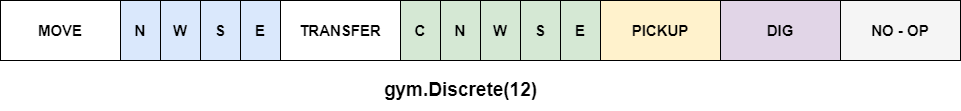
\includegraphics[width=1\linewidth]{images/methods_singleunit/action/controller.png}
    \captionsetup{justification=justified, singlelinecheck=false, width=1\linewidth, labelfont=bf} 
    \caption[]{The action space inside our controller included movements in four cardinal directions, transfers to four cardinal directions and center \protect\footnotemark, pickup, digging, and a no-operation action for debugging.}
    \label{fig:controller}
\end{figure}



\footnotetext{Transfer amount was set to the maximum available resource in cargo, circumventing binning or continuous bounded variables. The same rule applies for pickup actions as well.}


\noindent \textcolor{deepblue}{\autoref{fig:controller}} illustrates the action space adopted for our benchmarking analysis. We excluded certain operations available in the engine, including self-destruct, recharge, action queues (planning), and the transfer of resources other than Ice. The chosen action needed to be formatted to meet the specifications required by the Lux Engine, as detailed in \textcolor{deepblue}{\autoref{fig:lux-actions_ex}}.

\subsection{Observation}
\label{subsec:single-observation}

\noindent Our observation feature space was also designed with simplicity in mind, consisting of only a one-dimensional vector tailored specifically to the task of Ice mining. We intentionally excluded complex data types such as image maps, text, and extensive global information and conducted a small focused \textbdd{ablation study} to make sure the most significant features are present in the input space of the model. As shown in (\textcolor{deepblue}{\autoref{fig:feature-space}}), the features can be broken down into three components. The first section is the unit vector, which contains information about the state of the agent. Namely, the agent's position, class, team, and cargo data. The other two categories are observations about the environment itself. The features included here are vectors pointing towards the closest factory or ice tiles.

\begin{figure}[htbp]
    \centering
    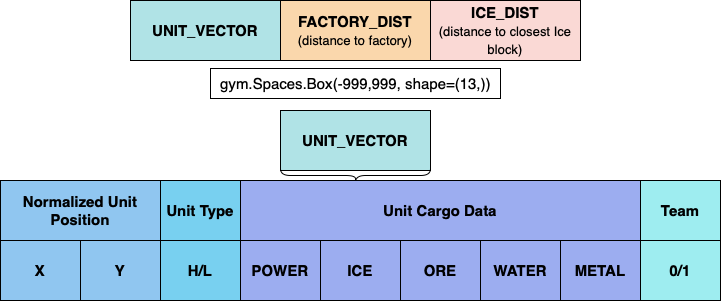
\includegraphics[width=0.8\linewidth]{images/methods_singleunit/observation/feature_space.png}
    \captionsetup{justification=justified, singlelinecheck=false, width=1\linewidth, labelfont=bf} 
    \caption[]{The feature space specifically optimized to maximize Ice collection.}
    \label{fig:feature-space}
\end{figure}

\subsection{Network Architecture}
\label{subsec:single-network}

\noindent Our neural network architecture was also designed with efficient computation and speed in mind, incorporating a small \textbdd{multilayer perceptron (MLP)} with two hidden layers. Each layer uses one \textbdd{linear projection} followed by a \textbdd{ReLU nonlinearity}. The final output layer is a linear projection that maps to the action space of the environment. We evaluated eight state-of-the-art reinforcement learning algorithms: ARS, A2C, DQN, PPO, QR-DQN, R-PPO, TRPO, and MPPO, each utilizing distinct learning approaches and objectives for the agent. Some algorithms employ an actor-critic approach with distinct policy and value heads learned concurrently, while algorithms like DQN and QR-DQN focus on trying to estimate Q-values in different ways for state-action pairs. In contrast, ARS does not learn values, Q-values, or policies directly.

\bigskip

\noindent On-policy actor-critic algorithms often employ \textbdd{separate feature extractors} for the actor and critic components when utilizing simple network architectures like MLPs. This approach is computationally manageable even with relatively small state spaces and has been shown to yield better results (\textcolor{deepblue}{\cite{andrychowicz2020matters}}). However, for more complex models that require a CNN backbone, a shared network architecture should be used since it enables the sharing of critical features between the actor and critic heads while significantly reducing computational overhead. 

\bigskip

\noindent Value-based methods and ARS utilized \textbdd{shared feature extractors}, as they focused solely on learning only Q-values, quantiles, and policy, without the need for distinct learning objectives such as separate value or policy heads. However, not all value-based methods follow this pattern. For instance, Double Deep Q-Learning (\textcolor{deepblue}{\cite{vanhasselt2015deep}}) employs two distinct networks: a primary online network for continuous learning and decision-making, and a separate target network, which is a clone of the primary network. The target network serves as a stable benchmark and is updated less frequently than the primary network.

\bigskip

\noindent It is important to note that while Stable Baselines 3 adheres to the specifications outlined in original research papers (\textcolor{deepblue}{\cite{stable-baselines3}}), these documents often omit significant implementation details, necessitating cautious interpretation of results (\textcolor{deepblue}{\cite{shengyi2022the37implementation}}). Moreover, Stable Baselines 3 incorporates significant, occasionally redundant, code overhead. This issue became more apparent when we used a single-file implementation of the PPO algorithm (\textcolor{deepblue}{\cite{huang2022cleanrl}}), to which we introduced several optimization techniques. For this benchmark study, we are continuing with the SB3 baselines.

\begin{figure}[htbp]
    \centering
    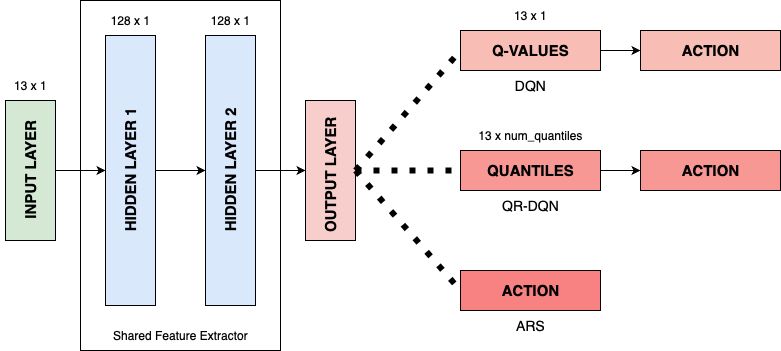
\includegraphics[width=0.8\linewidth]{images/methods_singleunit/net/shared_policy.png}
    \captionsetup{justification=justified, singlelinecheck=false, width=1\linewidth, labelfont=bf} 
    \caption[]{A high-level overview of the neural network layout that employs shared feature extractors used for value-based methods: DQN, QR-DQN, ARS.}
    \label{fig:shared-policy}
\end{figure}

\begin{figure}[htbp]
    \centering
    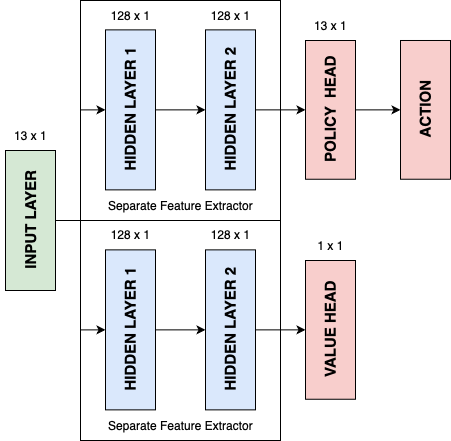
\includegraphics[width=0.6\linewidth]{images/methods_singleunit/net/separate_policy.png}
    \captionsetup{justification=justified, singlelinecheck=false, width=1\linewidth, labelfont=bf} 
    \caption[]{A high-level overview of the neural network layout that employs separate feature extractors used for actor-critic-based methods: A2C, PPO, TRPO, M-PPO, R-PPO. It's important to note that in our implementation of Recurrent Proximal Policy Optimization (R-PPO), we opted for two LSTM layers with a hidden size of 128, instead of using traditional linear projection layers due to the recurrent nature of the algorithm.}
    \label{fig:separate-policy}
\end{figure}


\subsection{Reward Function}
\label{subsec:single-reward}

\noindent Lastly, our reward system was designed with heavy shaping to incentivize two specific behaviors. It encouraged the agent to increase Ice collection and motivated the factory to produce more Water than in the previous round. \textbdd{This 1-step lookback} update-based reward system proved to be an effective method for encouraging targeted behaviors within our model.

\begin{equation}
    r_t = \frac{\Delta \text{ } ice\_dug}{100} + \Delta \text{ } water\_produced
    \label{eq:reward-function}
\end{equation}


\subsection{Training}
\label{sec:single-unit-training}

\noindent We ensured uniformity across all training environments for the algorithms discussed by adhering to the following paradigms:

\begin{itemize}[itemsep=4pt, parsep=0pt]

\item Each algorithm was tested across \textbdd{three trials}, training each from scratch.

\item A \textbdd{specific seed} was manually set for all algorithms and the SB3 torch configuration to maintain consistency across runs.

\item We utilized 8 parallel environments all running on different threads of our CPU.

\item Each environment was configured with a \textbdd{fixed rollout size of 8,192 steps} for policy gradient algorithms, ensuring consistent evaluation across iterations. For value-based methods, the \textbdd{target network was updated every 8,192 steps} to maintain stability. Additionally, each episode was allowed to extend up to 1,024 steps without any truncation. For ARS, updates were calculated at every step.

\item The enemy player was configured as a passive entity without decision-making capabilities; their water count was set to a high level to prevent their factory from being destroyed. Consequently, during each training step, the model was updated using data from \textbdd{only one team}.

\item The predefined hyperparameter sets from the original stable baselines repository were utilized for all algorithms. Batch size was adjusted to 1,024 for all algorithms except ARS, which does not utilize batch updates, in order to accommodate larger updates. Additionally, the \textbdd{number of gradient updates was set to 10} per training phase for all algorithms, with the exception of ARS.

\item A shared feature extractor architecture was employed across all algorithms, consisting of an MLP with two linear layers of size 128 and two ReLU activation layers.

\item All trials were conducted up to a total of \textbdd{1,000,000 steps} (1M).

\end{itemize}


\subsection{Evaluation}
\label{sec:single-unit-eval}

\noindent Our objective in evaluating these novel algorithms was to select one of the eight for scaling up and further assessments across various agent control levels. We aimed to identify an algorithm that aligns best with our specific problem, offers quick performance to speed up research progress, and delivers promising metrics in our benchmark study. The algorithms underwent continuous online evaluation, with the agent interacting with the environment in alternating training and evaluation phases. The criteria for the evaluation phases were as follows:

\begin{itemize}[itemsep=4pt, parsep=0pt]
    \item Every 8,192 steps, four parallel environments were instantiated with a \textbdd{limit of 1,000 maximum episode steps}, the usual game length in the Lux environment.
    
    \item After each evaluation phase, the model state was saved. If it performed better than the current best, the evaluation step was updated and saved.
    
    \item The same stochastic policy used during the training phase was employed for the evaluation phase, meaning that actions were chosen probabilistically rather than greedily at each step.
    
    \item Twelve evaluation episodes were conducted at every phase, resulting in $4 \times 12$ full runs of evaluation episodes to 1,000 maximum episode steps.
    
    \item \textbdd{Quantitative evaluations} utilized metrics that assessed the agent's performance in the environment, such as \textbdd{ice dug} and 
    \textbdd{ice transferred}. These metrics were calculated as the average over the $4 \times 12$ environments.
    
    \item The final quantitative results were averaged over all three trials, meaning the plotted results represent an average over $3 \times 4 \times 12$ evaluation episodes at every 8,192 step interval.
    
    \item Speed (\textbdd{step per second}) was used as an auxiliary metric to measure what could be expected from the algorithms if scaled up.
\end{itemize}

\noindent Our analysis showed conclusive results, identifying Masked-PPO as the most effective algorithm across several metrics: it achieved convergence in the fewest steps, exhibited the fastest performance among the algorithms that actually converged, and its application in multi-agent tasks has been widely documented. Its design allows for straightforward CPU and GPU parallelization due to fixed rollout lengths and minibatch updates. Consequently, Masked Proximal Policy Optimization (M-PPO) will be the primary focus of our subsequent research, while other algorithms may be revisited in future studies.

\section{Multi Agent Environment}
\label{sec:multi-agent-environment}

\noindent Having \textbdd{more than one non-heuristically controlled entity} brings up the question: What do we call an agent? The team of entities, or the entities that make up that team? The Lux Environment (\autoref{sec:environment}) presents a unique challenge in multi-agent control due to its diverse entity types: factories and units. These entities have distinct action spaces and characteristics. Units can be further categorized into light and heavy units, each with different strengths and weaknesses. Units are created by the factories, which further complicates the situation since the \textbdd{number of entities depends on the entities' actions} themselves, and these numbers are \textbdd{constantly changing}.

\bigskip

\noindent In our work, we explored various agent-control approaches, mainly \textbdd{centralized} architectures, where a single pass through the model is responsible for selecting actions for the entire team, turning the multi-agent scenario into a single-agent problem where each controllable entity becomes part of a complex composite action space. One of such implementations is our \textbdd{monolithic approach} (\autoref{sec:monolithic-approach}), where the agent makes decisions for every entity based on a global observation. However, as we will later discuss, this method requires the agent to \textbdd{interpret the entire game state}, which is particularly challenging in highly dynamic environments such as Lux. The complexity of this environment highlights the limitations of existing approaches and the need for a new, more adaptable solution.

\bigskip

\noindent Instead of using a single pass through a centralized model, another option would be to generate actions for every entity individually, based on their own observations. Generating a single entity's action massively reduces the required complexity of the network. Furthermore, we can treat each entity as a \textbdd{separate, parallel environment trajectory}, increasing the train examples collected from one step of the environment. Solutions for PettingZoo ({\cite{terry2021pettingzoo}}) multi-agent environments have been successfully trained with similar approaches using SuperSuit (\cite{SuperSuit}). However, \textbdd{changing agent numbers} poses a problem for such implementations. In our case, factories can explode throughout the game, and units are frequently destroyed or created, making existing multi-agent training solutions obsolete for our use case because they assume a constant number of agents throughout the episode. Additionally, training with on-policy methods requires \textbdd{careful tracking of their trajectories} and creates \textbdd{constantly changing batch sizes} if we treat every agent as a separate observed step. The Lux Environment can have hundreds of units active simultaneously. Storing observations and calculating actions for each unit and factory \textbdd{hinders performance at both training and inference}. For these reasons, we have not explored full multi-agent control. Instead, we used what we call a \textbdd{hybrid approach} (\autoref{sec:hybrid-approach}), which uses a \textbdd{centralized decision-maker} while allowing \textbdd{individual control} of units and factories based on both \textbdd{local and global information}.

\section{Monolithic Approach}
\label{sec:monolithic-approach}

\noindent In our monolithic solution, we introduce a \textbdd{central decision-maker} agent, serving as the exclusive learning entity with oversight over entities that provide information but lack \textbdd{direct influence} on the whole learning process. This framework enables the central decision-maker to supervise all units on the map concurrently, leveraging a global trajectory and reward system for updates. To tackle the challenge of fluctuating numbers of learning agents (\cite{piccoli2023control}; \cite{SuperSuit}), such as factories or units, we implemented a \textbdd{single-trajectory approach} for each episode. This method ensures fixed episode lengths, independent of factors like unit deaths or creations, resulting in a singular termination flag at the conclusion of each episode.

\bigskip

\noindent In our context, \textbdd{direct influence} refers to the scenario where the actions of a single entity directly impact the central decision-maker. However, in the case of the monolithic approach, this direct influence does not occur. Instead, the central brain only perceives global changes in the environment without attributing them to specific agents. We refer to this as \textbdd{indirect influence} on the learning agent. This distinction significantly simplifies the functioning of the learning agent. For instance, when there is a positive change in the environment, such as ice collection, it is reinforced without the need to identify which agent was responsible for the action.

\bigskip

\noindent In our approach, we utilize a single actor and a single critic, forming a \textbdd{single-task learning setup} (\cite{eysenbach2023connection}; \cite{gai2024singletask}; \cite{mysore2022multicritic}) that optimizes a unified global objective. The single actor generates actions for every pixel on the map, creating a global action tensor that encompasses the entire map. From the raw observations, we filter out pixels containing units and factories to form a tensor of shape $M\times|A|$, where $M$ is the number of factories and units, and $|A|$ represents the size of the action space. Similarly, the single critic approximates the singular value of the entire game state. This is what we refer to as a \textbdd{monolithic framework} for PPO: it includes global observations, a single decision maker, a single global trajectory for every episode, a global reward system, a single actor generating a global action tensor, and a single critic evaluating the global state of the game.

\subsection{Environment}
\label{subsec:mono-environment}

\noindent There were minor changes to the environment and learning setups compared to \autoref{sec:single-unit-testbench}. We expanded the action space to include the \textbdd{recharge action} for units and \textbdd{three additional factory actions}: light unit building, heavy unit building, and lichen watering. This adjustment increased the original discrete action space (\autoref{subsec:single-environment}) from 12 to 16. Additionally, we implemented more rigorous action masking, which restricted units from transferring resources to enemy units and factories, prevented out-of-bounds movements, and limited factory unit generation.

\bigskip

\noindent We reduced the episode length during the training phase to 256 steps to \textbdd{fit a broader range of data within the same number of training examples}. This adjustment was driven by the observation that the environment dynamics stabilize after a certain number of steps, especially when the goal is to sustain the factories. Given the relatively straightforward strategy of mining ice and transporting it to the factory, the mechanics remain largely consistent throughout the match. By shortening the episode length during training, we were able to parallelize more environments, resulting in accelerated training.

\subsection{Heuristic Bidding and Factory Placement}
\label{subsec:heur-bidding-factory}

\noindent In our experiments, we aimed to  \textbdd{minimize variance between environments} by employing heuristics for the bidding and factory placement phase (\autoref{subsec:early-game}). Given that bidding reduces starting resources, leading to faster factory depletion, we consistently bid with zero. To optimize ice supply to factories, we identified locations where the \textbdd{adjacency of ice to factories is maximal}. \textbdd{Gaussian filtering} (\cite{gaussianfilter}) techniques were applied to the board to smooth out data, emphasizing nearby points and reducing noise. Gaussian filtering is a method that smooths out data, like images or, in our case, an observed matrix of the board, by giving more importance to nearby points in a \textbdd{bell-shaped distribution}, reducing noise and sharp transitions. This effectively causes the values on the board to spread out in an area, indicating how far away a tile is from other relevant tiles  as shown on Figures \ref{fig:grad-image} to \ref{fig:gaussian-rubble}. After applying Gaussian filtering, the smoothed boards are weighted and summed pixel-wise to obtain final scores for each tile. Placement selection is then performed \textbdd{greedily}, with the factory placed on the tile with the highest score among the currently valid placement locations (\autoref{fig:score-map}).


\begin{figure}[htbp]
    \centering
    \begin{minipage}{1\textwidth}
        \centering
        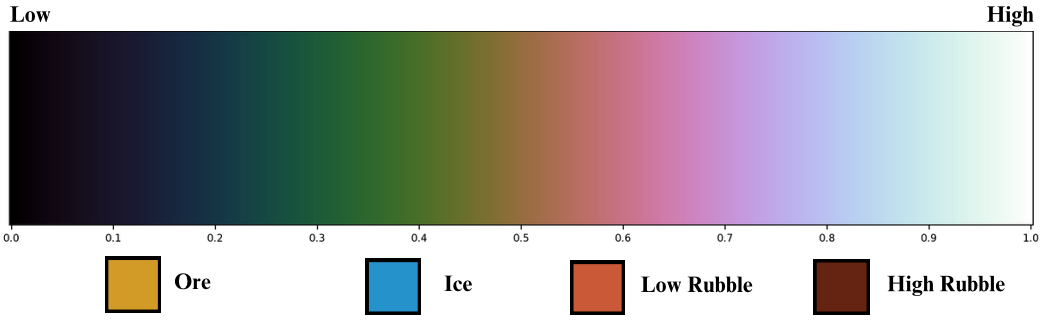
\includegraphics[width=0.8\linewidth]{images/methods_mono/factory_placement/grad.png}
        \captionsetup{justification=justified, singlelinecheck=false, width=1\linewidth, labelfont=bf} 
        \caption{The legend image provided below accompanies subsequent images. It illustrates the original starting map of the Lux environment. The gradient color scheme represents the presence of elements, with lighter colors indicating lower presence and darker colors indicating higher presence. The color mapping for ore, ice, and rubble remains consistent with previous representations (\autoref{fig:lux-map}).}
        \label{fig:grad-image}
    \end{minipage}\hfill
    \centering
    \begin{minipage}{1\textwidth}
        \centering
        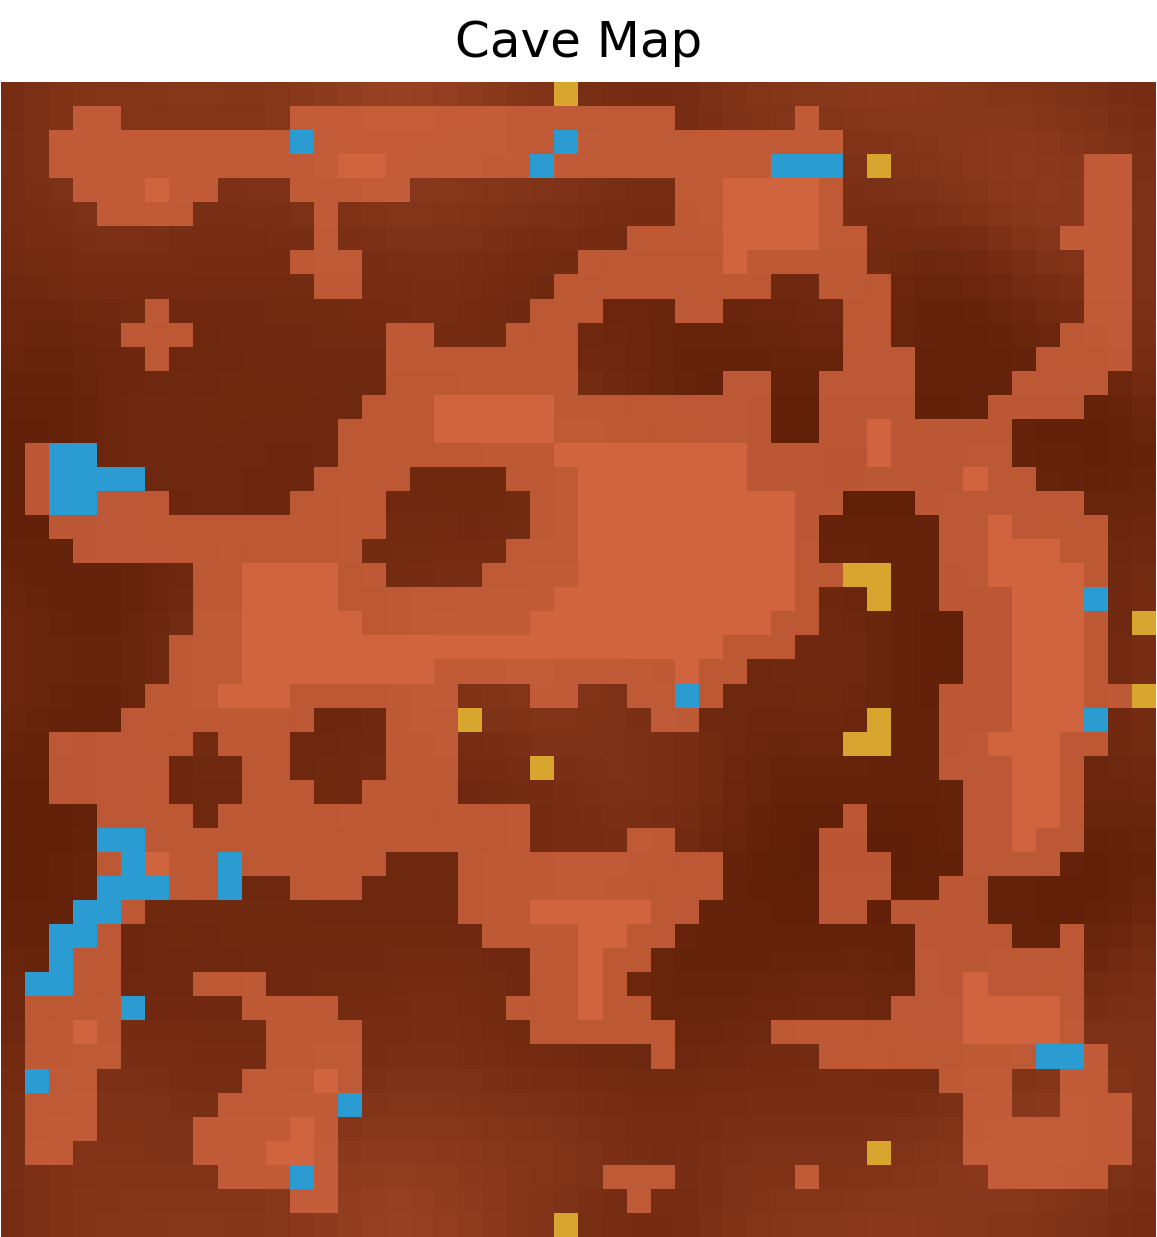
\includegraphics[width=0.3\linewidth]{images/methods_mono/factory_placement/cave_map.png}
        \captionsetup{justification=justified, singlelinecheck=false, width=1\linewidth, labelfont=bf} 
        \caption{Image of the original starting seed of the map without any factories placed on it, generated as the initial step before the bidding phase.}
        \label{fig:grad-map}
    \end{minipage}\hfill
    \vspace{8pt}
    
    \begin{minipage}{0.3\textwidth}
        \centering
        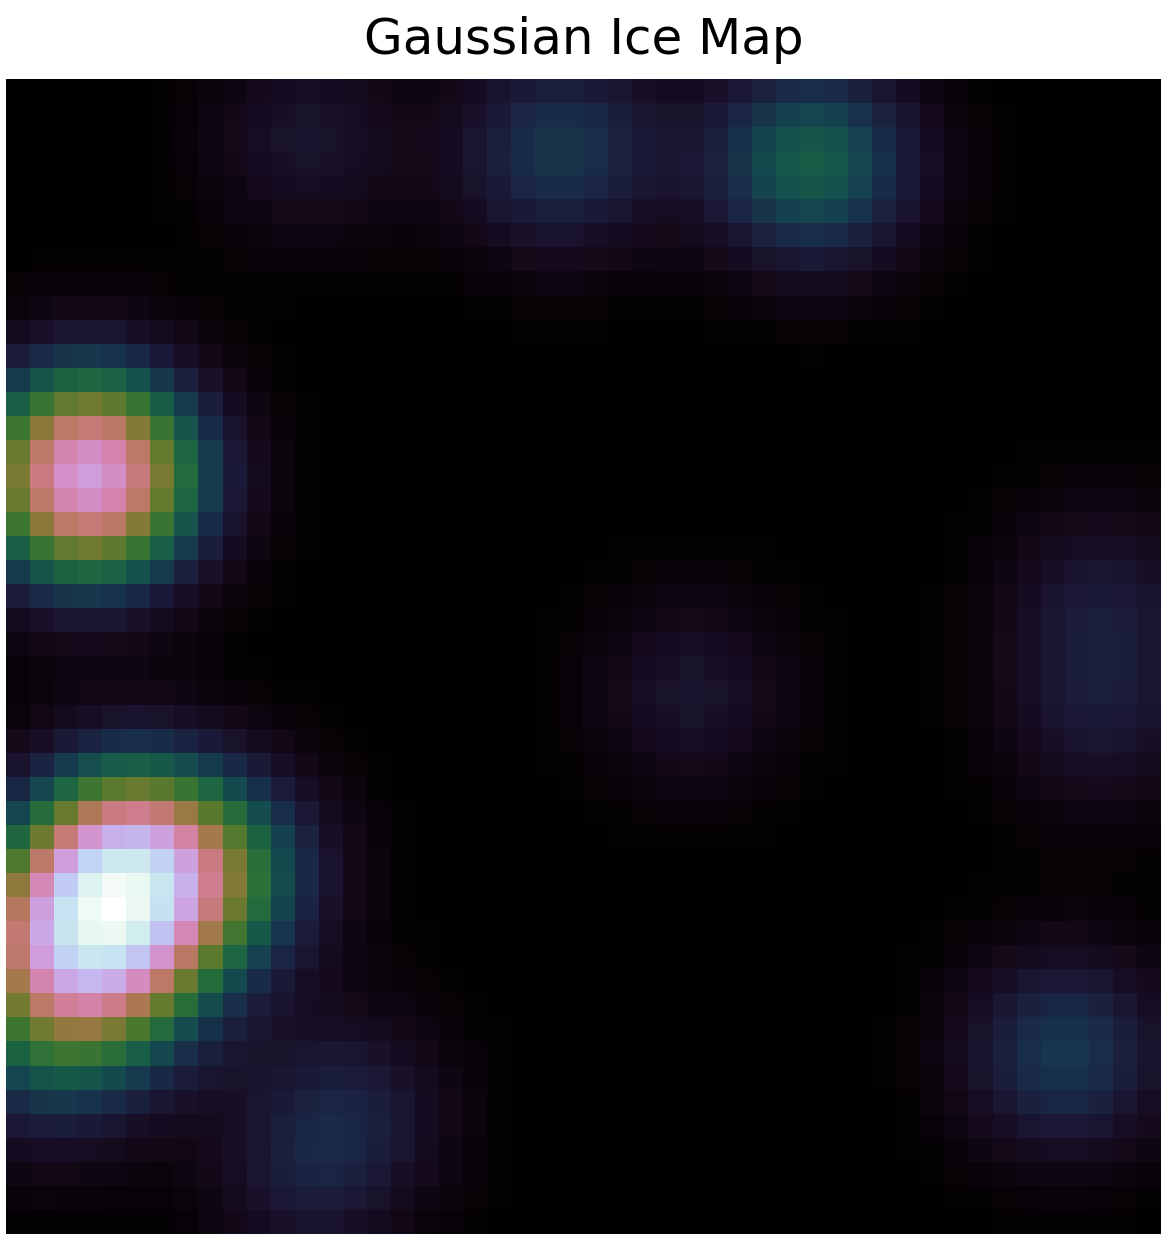
\includegraphics[width=\linewidth]{images/methods_mono/factory_placement/gaussian_ice_map.png}
        \captionsetup{justification=justified, singlelinecheck=false, width=1\linewidth, labelfont=bf} 
        \caption{High presence of ice calculated using our Gaussian filter. Lighter values indicate high-density ice areas.}
        \label{fig:gaussian-ice}
    \end{minipage}\hfill
    \begin{minipage}{0.3\textwidth}
        \centering
        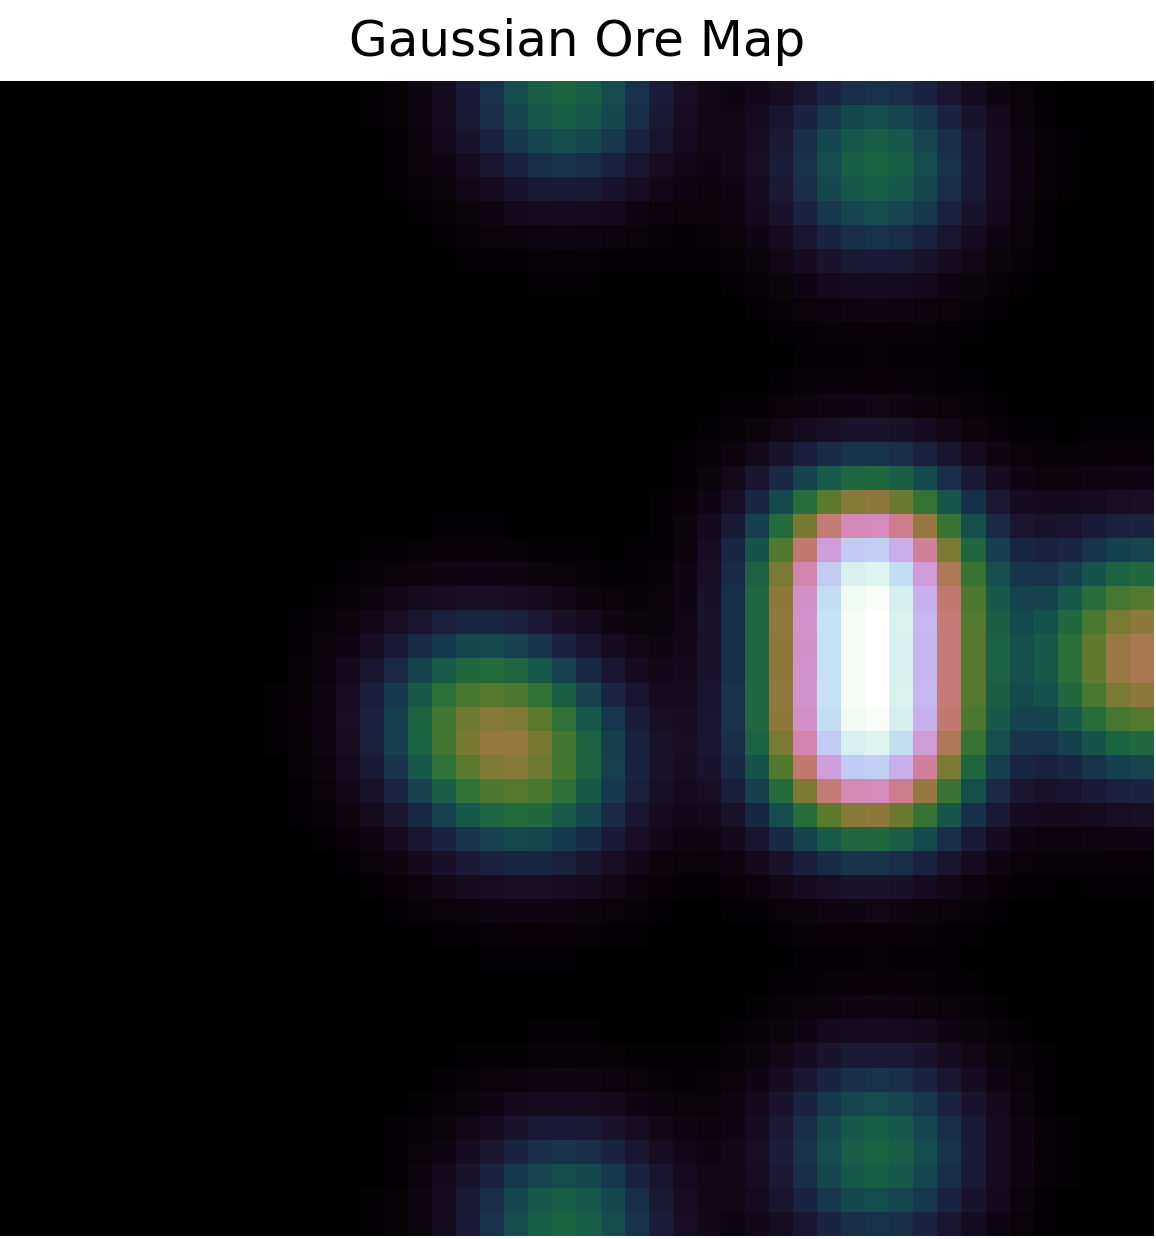
\includegraphics[width=\linewidth]{images/methods_mono/factory_placement/gaussian_ore_map.png}
        \captionsetup{justification=justified, singlelinecheck=false, width=1\linewidth, labelfont=bf} 
        \caption{High presence of ore calculated using our Gaussian filter. Lighter values indicate high-density ore areas.}
        \label{fig:gaussian-ore}
    \end{minipage}\hfill
    \begin{minipage}{0.3\textwidth}
        \centering
        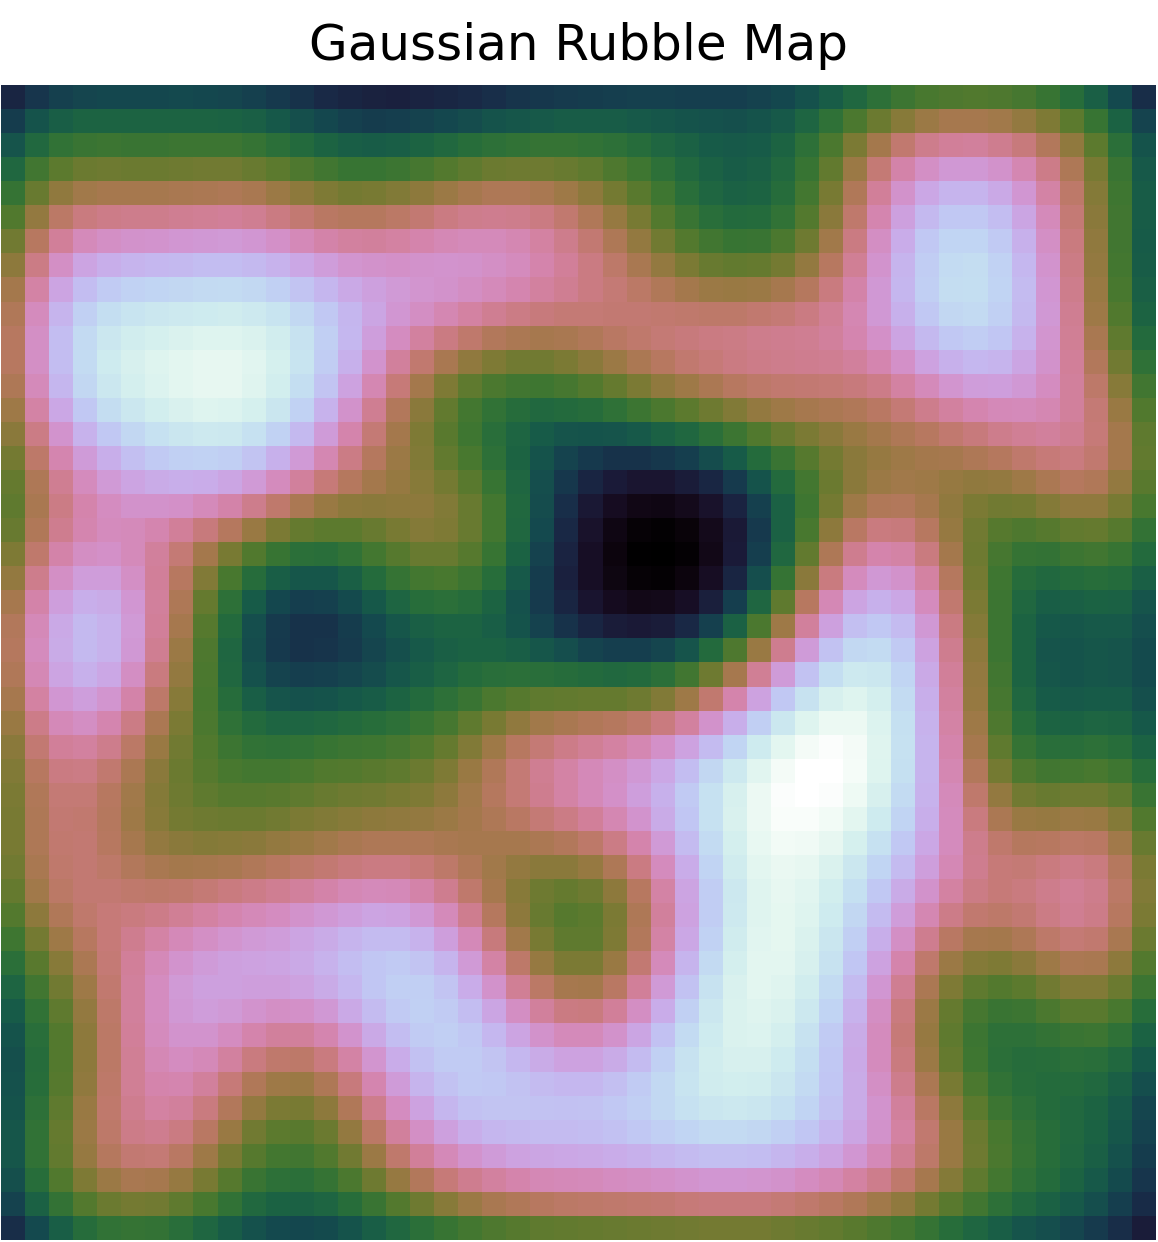
\includegraphics[width=\linewidth]{images/methods_mono/factory_placement/gaussian_rubble_map.png}
        \captionsetup{justification=justified, singlelinecheck=false, width=1\linewidth, labelfont=bf} 
        \caption{High presence of rubble calculated using our Gaussian filter. Lighter values indicate high-density rubble areas.}
        \label{fig:gaussian-rubble}
    \end{minipage}
\end{figure}


\begin{figure}[htbp]
    \centering
    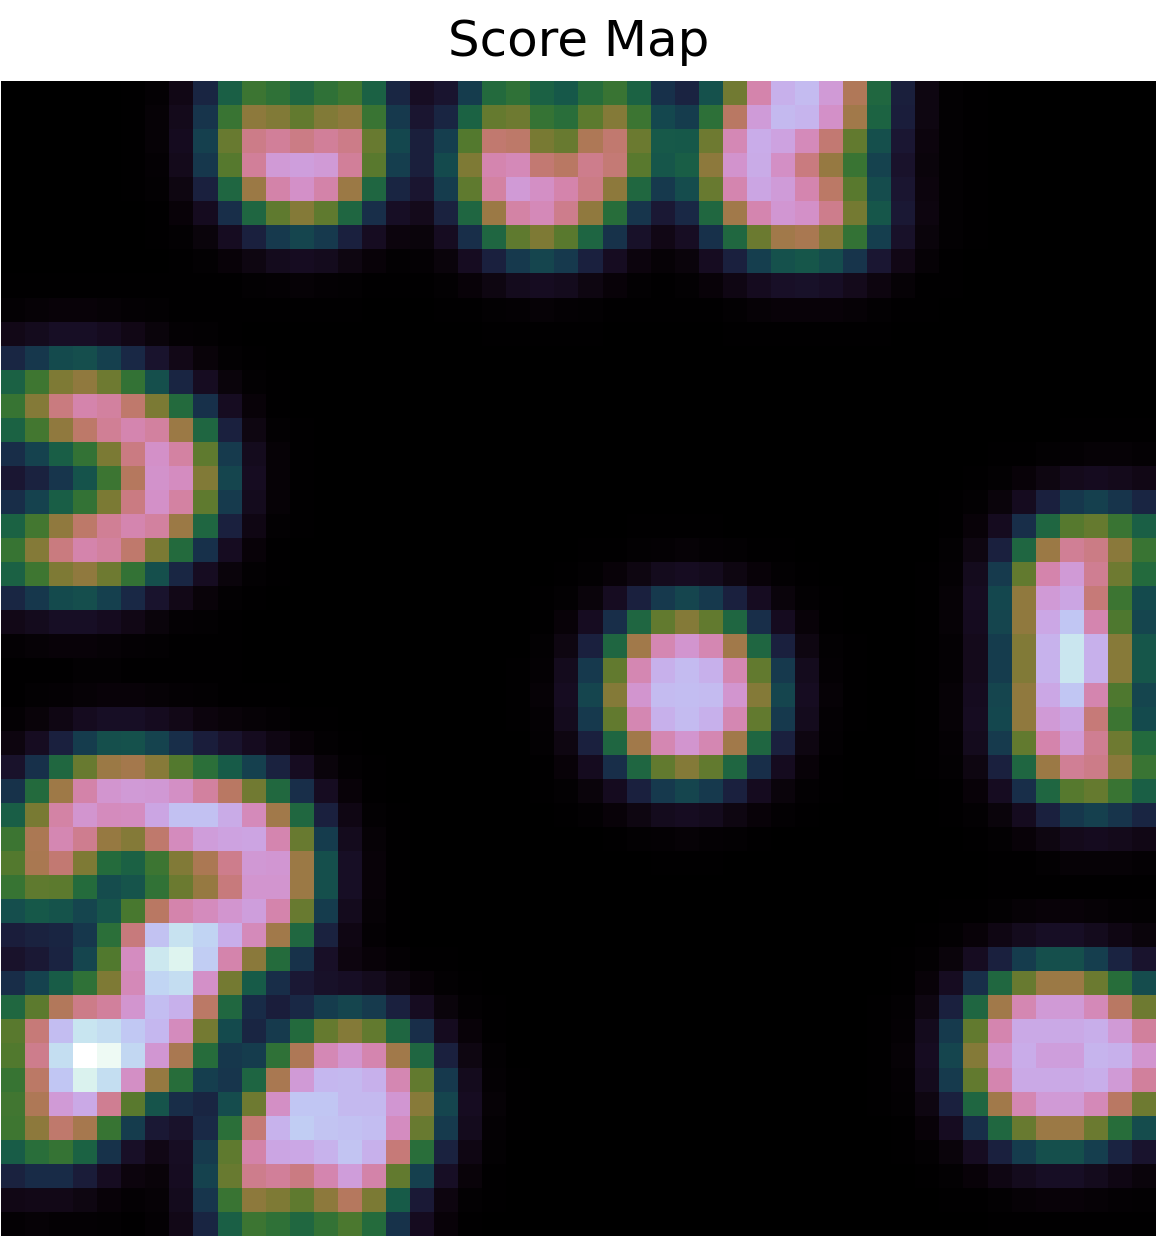
\includegraphics[width=0.3\linewidth]{images/methods_mono/factory_placement/score_map.png}
    \captionsetup{justification=justified, singlelinecheck=false, width=1\linewidth, labelfont=bf} 
    \caption[]{The output of the Gaussian filter algorithm applied to the ore, ice, and rubble maps weighted with possible spawn position maps \protect\footnotemark. Lighter areas indicate the best possible spawn locations.}
    \label{fig:score-map}
\end{figure}

\subsection{Actions}
\label{subsec:mono-actions}

\noindent Utilizing a single actor, we compressed our action space into a single discrete space, accommodating both unit and factory actions. To ensure precise probability calculations and to restrict factory actions for units, and vice versa, we \textbdd{employed invalid action masks}. This essentially led to a theoretical \textbdd{splitting of the action space} into two categories: factory actions and unit actions. Factory actions were masked out for all units, and unit actions were masked out for all factories, with the exception of the no-operation action, which was available to both entity types. Restricting illegal actions within such vast action spaces is crucial for expedited learning. For instance, by forbidding the transfer action when no cargo is available on the unit or when the unit is not adjacent to another unit, or when the factory is not adjacent to the unit, we effectively reduced the range of possible unit actions from 13 to 8 (including move in 4 cardinal directions, pickup, dig, recharge, and no-operation) (\autoref{subsec:lux-action}). Although we did not implement a more complex masking system to limit repeated actions or prevent agents from overlapping, as it would introduce excessive logic and determinism into the game, we aimed for the central decision maker to \textbdd{learn these patterns} rather than explicitly instructing it on all possible negative edge cases. Lichen watering was also excluded for all factories to better align them with the task of preserving their longevity, as watering lichen consumes water, thereby reducing factory lifespan. For global control, our final action space was of size $[16,48,48]$, where each pixel on the map had an assigned action vector, as illustrated in \autoref{fig:action_space_mono}.

\footnotetext{The possible spawn positions are represented by a mask matrix where True values indicate valid spawn positions and False values indicate invalid ones. Invalid positions for factories include those on top of ore blocks, ice blocks, or the very edges of the map. This information is provided and calculated by the Lux AI engine.}

\begin{figure}[htbp]
    \centering
    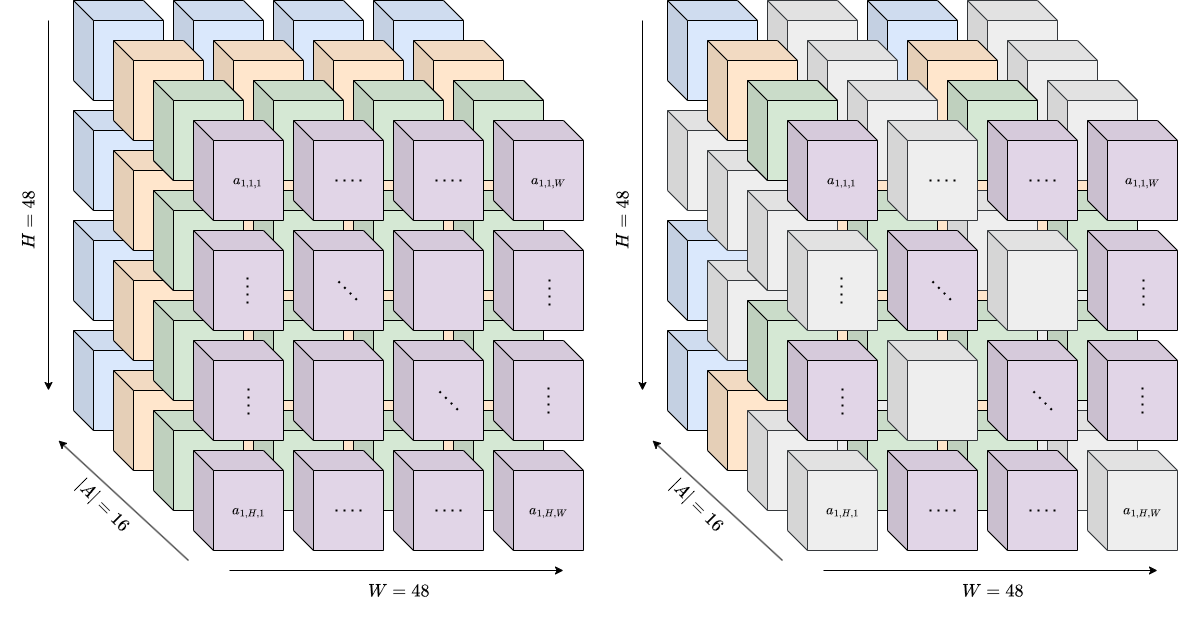
\includegraphics[width=0.7\linewidth]{images/methods_mono/action/action_space.png}
    \captionsetup{justification=justified, singlelinecheck=false, width=1\linewidth, labelfont=bf} 
    \caption[]{A comprehensive representation of an action tensor is depicted on the left, alongside its masked version utilizing invalid action masking. Here, \textbdd{masked out} refers to actions that are deemed invalid in the environment given a state $s$. Similarly, colored boxes indicate the same actions across different pixels of the environment. This representation has limitations, as it shows each pixel on a $4\times4$ grid with $4$ possible actions each. From the illustration, it is also visible that invalid action masking effectively reduces the exploration space of the environment for the learner agent.}
    \label{fig:action_space_mono}
\end{figure}



\subsection{Observation}
\label{subsec:mono-observation}

\noindent The observation features were also overhauled from the single-unit testbench (\autoref{subsec:single-observation}), aiming to create a compact observation space while still providing the model with all relevant information. These features can be categorized into four groups: \textbdd{global features, map features, unit features, and factory features}. Global features consist of scalar values that are tiled to the shape of the map for concatenation with other features. Map, unit, and factory features are all shaped \textbdd{H x W}, where \textbdd{H} represents the game board's height and \textbdd{W} its width, describing the tile of the board, units, and factories respectively. Features are represented as 32-bit floating-point numbers. Boolean flags are converted to zeros and ones, while other values are normalized to a \textbdd{[-1, 1] range}. This normalization ensures that the mean of the inputs are close to zero, aiding convergence (\cite{Normalization}). All features are concatenated as channels into a single tensor within the model. See \autoref{tab:features} for a complete list of features.

\bigskip

\noindent The model additionally receives two matrices, each cell containing the ID of the unit or factory occupying that position on the map, representing the entity's team affiliation. These matrices do not alter entity behavior but are utilized during training for reward assignment, critic values, log probabilities, and entropy values. Further details on reward assignment will be provided in \autoref{subsec:grouping}.

\begin{table}[htbp]
    \centering
    \begin{tabular}{|c|c|c|c|}
        \hline
        \textbf{Feature Type} & \textbf{Feature Name} & \textbf{Shape} & \textbf{Value Range} \\
        \hline
        Global & Step & Scalar & [-1, 1] \\
        Global & Daytime & Scalar & \{0, 1\} \\
        \hline
        Map & Friendly Factory & H x W & \{0, 1\} \\
        Map & Ice & H x W & \{0, 1\} \\
        Map & Ore & H x W & \{0, 1\} \\
        Map & Rubble & H x W & [-1, 1] \\
        Map & Friendly Unit & H x W & \{0, 1\} \\
        Map & Enemy Unit or Factory & H x W & \{0, 1\} \\
        \hline
        Unit & Heavy Unit & H x W & \{0, 1\} \\
        Unit & Power in Battery & H x W & [-1, 1] \\
        Unit & Ice in Cargo & H x W & [-1, 1] \\
        Unit & Ore in Cargo & H x W & [-1, 1] \\
        \hline
        Factory & Power in Factory & H x W & [-1, 1] \\
        Factory & Ice in Factory & H x W & [-1, 1] \\
        Factory & Water in Factory & H x W & [-1, 1] \\
        Factory & Ore in Factory & H x W & [-1, 1] \\
        Factory & Metal in Factory & H x W & [-1, 1] \\
        \hline
    \end{tabular}
    \captionsetup{justification=justified, singlelinecheck=false, width=1\linewidth, labelfont=bf}
    \caption{Table containing the complete list of observation features, along with their shape and normalized value range. $H$ and $W$ refer to the height and width of the board.}
    \label{tab:features}
\end{table}

\subsection{Weight Scaling}
\label{subsec:weight-scaling}

\noindent The scaling factor of the weight initialization can have a substantial effect on the \textbdd{variance} of both the \textbdd{activations and the gradients} (\cite{pmlr-v9-glorot10a}). Proper weight initialization for the Rectified Linear Unit (ReLU) activation function with the scale of $\sqrt{\frac{2}{n_t}}$, where $n_t$ is the number of input units to the layer, has been shown to ensure \textbdd{zero mean and unit variance} of the outputs (\cite{DBLP:journals/corr/HeZR015}), stabilizing the learning process. Omitting the $n_t$ terms causes higher variance but has been widely used in practice, for which the original PPO implementation is a good example. Since we use Leaky ReLU activations, we employed the slightly modified scaling of \autoref{eq:gain}, which was the scaling recommendation for that specific activation in the Pytorch framework (\cite{pytorchinit}).

\begin{equation}
    \texttt{gain} = \sqrt{\frac{2}{1+\texttt{negative\_slope}^2}}
\label{eq:gain}
\end{equation}

\bigskip

\noindent Following the recommendations of \cite{shengyi2022the37implementation}, we used the activation function's recommended gain value as the scale for weight initialization in our hidden layers and a scale of 0.01 for the initialization of the actor head. We initialized the critic with the same scale to get \textbdd{predictions close to zero}, matching our scaled-down rewards (\autoref{subsec:hyb-rew}). After learning how much \textbdd{downscaling the weights} can help, in some benchmark tests boosting performance by 66\% (\cite{andrychowicz2020matters}), we further scaled down the output layers of the network by a factor of 100 to make the action distribution more closely resemble a \textbdd{uniform distribution}. We were still noticing fluctuations in performance based purely on the seed the networks were initialized with, so we performed the same scaling on the critic value output layer's weights and, eventually, the hidden layers.

\subsection{Feature Extractor Model}
\label{sec:monolithic-network}

\noindent We transitioned from a heavily shaped feature space to a \textbdd{CNN-based feature extractor}, aiming to map the observations detailed in section (\autoref{subsec:single-observation}) to an action tensor of size $[16, 48, 48]$. In this representation, 16 signifies the size of the discrete action space, while 48 denotes the map size. Given that both our observation tensor and action space possessed a channel size of 16, encompassing various map, unit, factory, and global features (\autoref{tab:features}), we required a mapping strategy to align the observation space with the action space structure (\autoref{sec:monolithic-network}). We implemented two distinct feature extractor architectures to achieve this goal.

\bigskip

\noindent The first network architecture adopted a U-Net style encoder (\cite{ronneberger2015unet}) with various variations of bottlenecks and a decoder with skip connections (\cite{wu2020skip}). U-Net architectures are well-known for their effectiveness in image segmentation tasks (\cite{ehab2023performance}; \cite{ronneberger2015unet}), and we aimed to achieve a similar outcome but at the \textbdd{entity level segmentation}. Our goal was for the network to recognize that entity-free spaces represented inactive segments of the input space, while units and factories remained segmented as distinct entities. Each entity's class corresponded to the action it performed in the environment. In simpler terms, we aimed to create a segmentation map that \textbdd{established a class system} for each agent, categorizing them into different classes. For instance, if the network predicted a dig action for a unit at a given pixel, it meant that the network had segmented it into a \textbdd{digger} class. Similarly, when the model predicted a recharge action, the corresponding agent was categorized into a \textbdd{recharger} class within the grid environment.

\bigskip

\noindent The encoder of the network employed \textbdd{Downsampling blocks}, transforming the input tensor from a shape of $[16, 48, 48]$ to $[256,3,3]$. Each Downsampling block comprised a residual block (\autoref{subsec:residual}) and a downsampling convolutional layer with a kernel size of 3 and a stride of 2, effectively \textbdd{halving} the height and width of its input. The residual blocks consisted of 2 convolutional layers, a squeeze-and-excitation layer (\autoref{subsec:se}), and a leaky ReLU (\autoref{subsec:leaky-relu}) as the residual, which was concatenated to the input of the residual block. Spectral (\autoref{subsec:spectralnorm}) and batch normalization (\autoref{subsec:batchnorm}) techniques were applied after each convolutional layer, followed by a leaky ReLU activation function.

\bigskip

\noindent Furthermore, each convolutional layer was initialized using orthogonal initialization techniques (\autoref{subsec:ortho}) following recommendations from the literature (\cite{shengyi2022the37implementation}). The weights have been further scaled down to minimize the fluctuations in performance between seeds that random initialization can cause (\autoref{subsec:weight-scaling}). To ensure reproducibility and \textbdd{reduce variation in different trial runs}, each layer was initialized with a combination of the global seed and the layer's unique hash. The Squeeze-and-Excitation module employed a reduction factor of 16, facilitating the calculation of channel weighting and importance for every input channel of the observation feature.

\bigskip

\noindent We explored various bottleneck architectures, including a \textbdd{simple convolutional bottleneck} comprising two residual blocks and and a \textbdd{multi-scale bottleneck} incorporating $1\times1$, $3\times3$, $5\times5$, and $7\times7$ convolution operations to expand the receptive field of the model (\cite{Gao_2021}). The multi-scale U-net architecture, in particular, aims to mitigate degradation issues in target regions of segmentation masks by creating representations of the input on different receptive fields and concatenating them to form a comprehensive feature space representation. This approach has been demonstrated to be effective in maintaining the integrity of target regions in segmentation tasks (\cite{article_bot}; \cite{zhu2024efficient}; \cite{bhojanapalli2020lowrank}). 

\bigskip

\noindent In the decoder component of the network, we designed upsampling blocks that mirrored the structure of the downsampling blocks but in reverse. Each upsampling block begins with a \textbdd{transpose convolution} (\cite{shelhamer2016fully}) to upsample the input feature map, followed by batch and spectral normalization and a leaky ReLU nonlinearity. The block concludes with a residual block, maintaining consistency with the previous structure. The inputs to the upsampling blocks consist of outputs from preceding layers and corresponding residuals from their paired downsampling blocks. We termed this feature extractor network the \textbdd{BottleNet} (\autoref{fig:BottleNet}).

\bigskip

\begin{figure}[htbp]
    \centering
    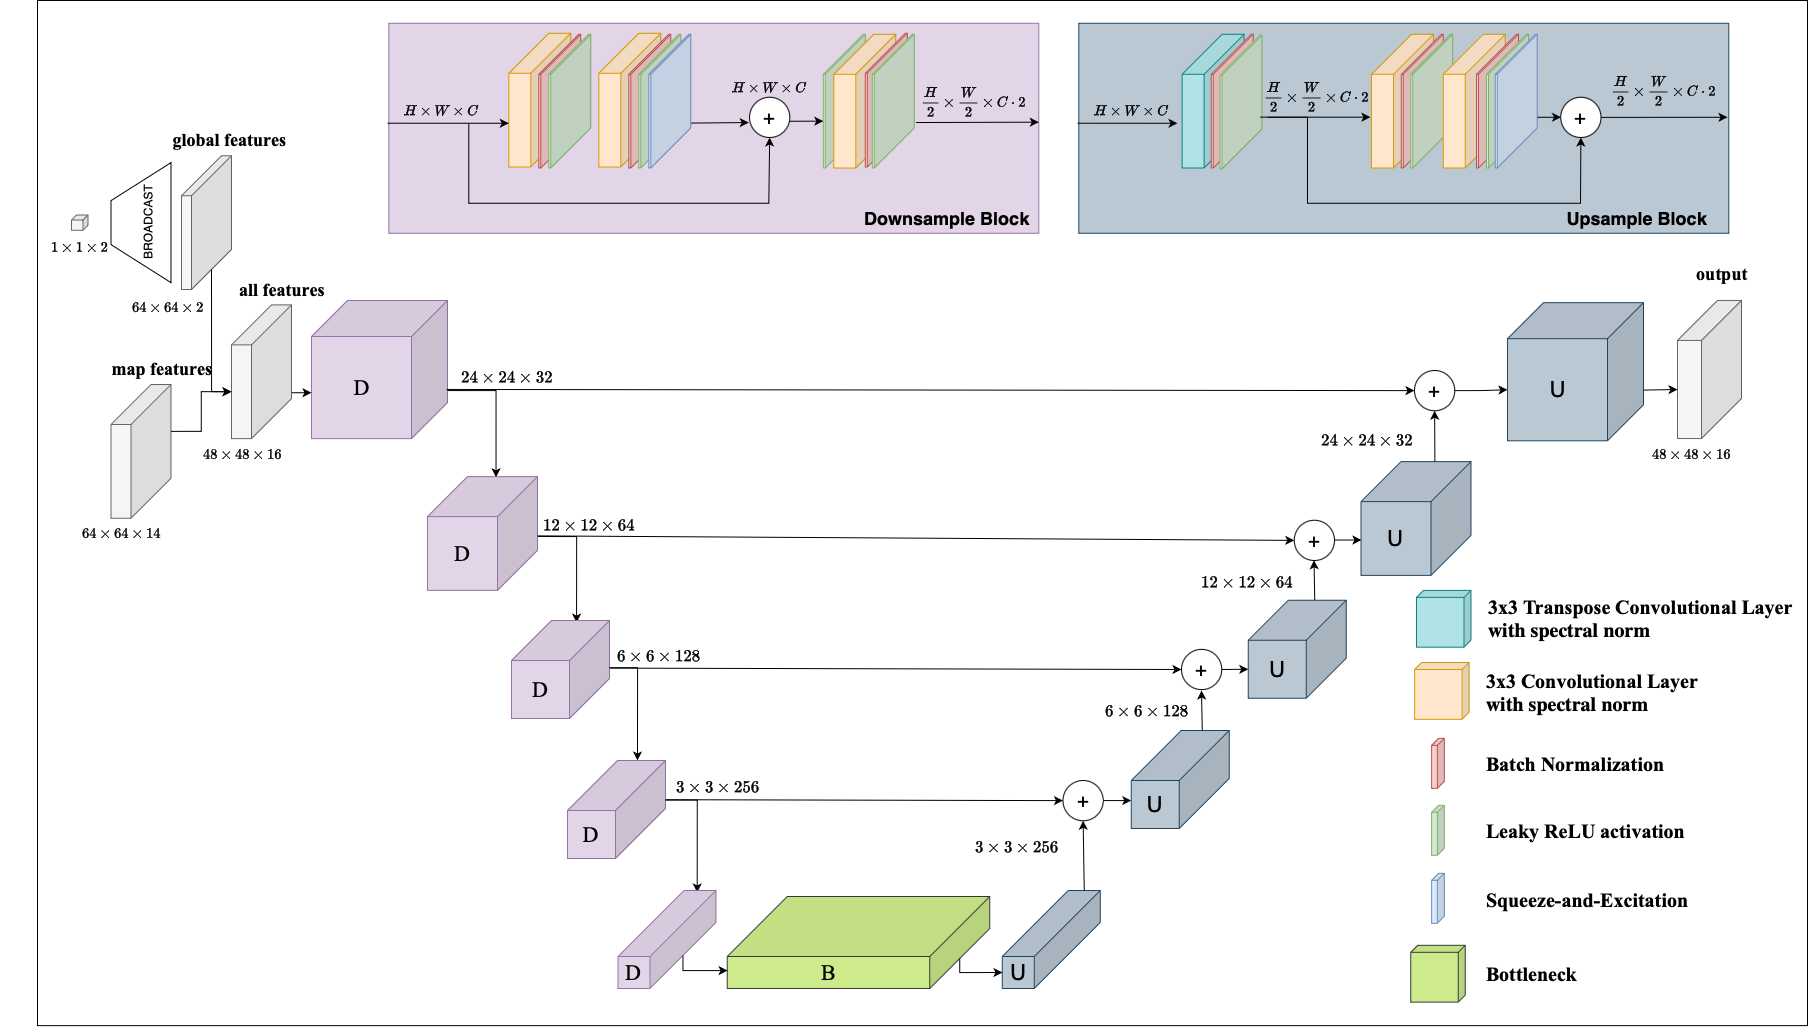
\includegraphics[width=0.9\linewidth]{images/methods_mono/feature_extractor/unet.png}
    \captionsetup{justification=justified, singlelinecheck=false, width=1\linewidth, labelfont=bf} 
    \caption[]{The figure depicts the entire feature extractor network, encompassing the process from input to output. Map features are combined with tiled-up global features, passing through a sequence of Downsample Blocks until reaching the bottleneck layer. The bottleneck layer's outputs are then upsampled via a series of Upsample Blocks, utilizing matching residuals from downsampling blocks to retain information. Finally, the output is directed towards both the critic and actor networks.}
    \label{fig:BottleNet}
\end{figure}

\begin{figure}[htbp]
    \centering
    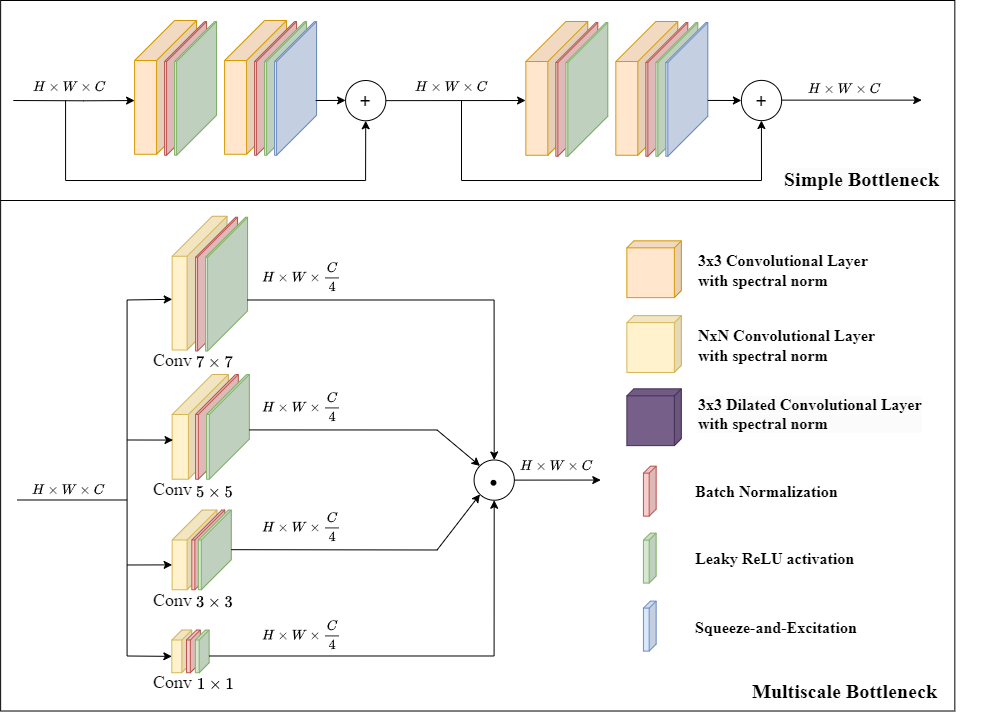
\includegraphics[width=0.8\linewidth]{images/methods_mono/bottleneck/bottleneck.png}
    \captionsetup{justification=justified, singlelinecheck=false, width=1\linewidth, labelfont=bf} 
    \caption[]{The three images illustrate various types of bottlenecks tested for our feature extractor. Starting from the top, the Simple Bottleneck consists of two residual blocks. The Dilated Bottleneck employs convolutional layers with dilation, where the filter expands by a certain factor, allowing it to capture a broader context. Lastly, the Multiscale Bottleneck features a four-branch network, emphasizing important features at different scales.}
    \label{fig:Bottlenecks}
\end{figure}


\noindent For our second network architecture, we opted to maintain the input and output sizes \textbdd{without downscaling}, thus eliminating bottleneck layers. With the goal of creating a one-to-one mapping, we designed a compact residual network that preserves the height and width of the feature maps throughout the network. This network comprises an input convolutional block with spectral normalization, batch normalization, and leaky ReLU nonlinearity. It is followed by four residual blocks, each incorporating SE layers for channel importance weighting, similar to the BottleNet architecture. The final block of this feature extractor network consists of another convolutional block with spectral normalization, batch normalization, and a leaky ReLU activation function. We named this feature extractor the \textbdd{DashNet}.

\subsection{Actor and Critic}
\label{sec:mono-network-actor-critic}

\noindent To ensure compatibility with Stable Baselines, we introduced an additional layer of feature extractor, separated for both the actor and policy networks. To simplify and reduce computational load, we applied a $3\times3$ convolutional layer to the output of our feature extractor network for the actor, incorporating batch, spectral, and layer normalization techniques. Then, for each pixel, its corresponding output value was sent through a linear projection layer, which mapped the extractor network outputs to action \textbdd{loglogits}. For the value network, to fully represent the value of the entire state from the output tensor, we used a single convolutional block paired with layer normalization and leaky ReLU nonlinearity. To refine the representation of value estimates, this mapping compressed the values into a more suitable space, enabling the inclusion of small negative values for more accurate estimates. Next, we employed a \textbdd{global average pooling method} \cite{lin2014network} to average the values of all pixels channel-wise, resulting in a 48x48-sized tensor. This tensor was then flattened and passed through a linear projection layer to produce the final value estimate (\autoref{fig:mono-actor-critic}).

\begin{figure}[htbp]
    \centering
    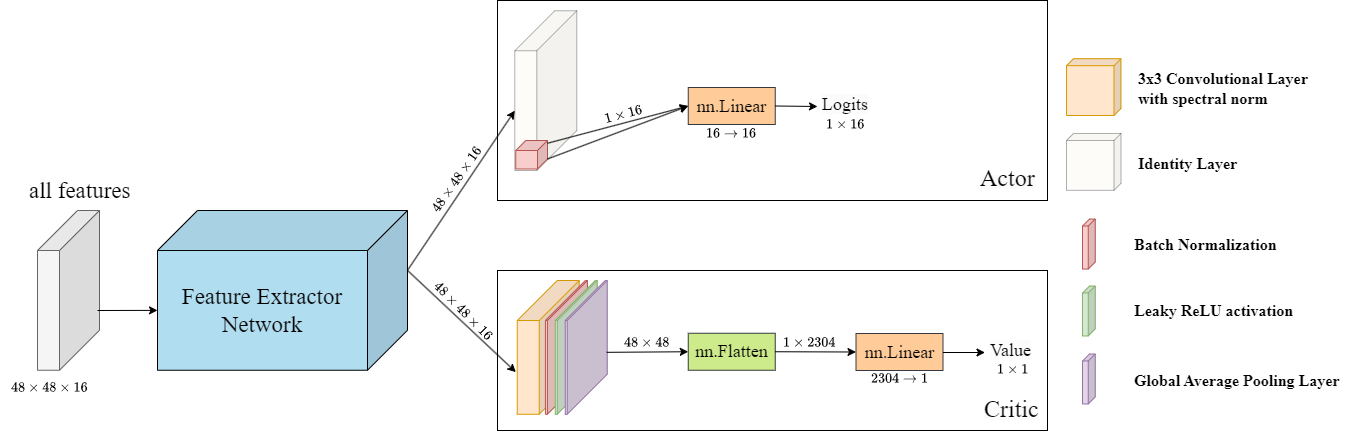
\includegraphics[width=1\linewidth]{images/methods_mono/actor_critic/actor-critic-head.png}
    \captionsetup{justification=justified, singlelinecheck=false, width=1\linewidth, labelfont=bf} 
    \caption[]{The diagram shows the actor and critic heads of the architecture. The actor head extracts action vectors for each pixel using an identity layer and a linear projection for logits. Meanwhile, the value head utilizes a final convolutional block with Global Average Pooling to calculate channel-wise averages, followed by a many-to-one linear projection.}
    \label{fig:mono-actor-critic}
\end{figure}

\subsection{Reward Function}
\label{sec:monolithic-reward-function}

\noindent We adjusted the rewards to incentivize global \textbdd{ice collection, ice transfer, and water generation} in the environment. Ice collection was scaled down by a factor of four to normalize its value to that of water (as 4 ice can be turned into 1 water by the factory). Additionally, we further downscaled the ice collection by a tenth to incentivize not only the digging of ice but also its transfer to factories, which was rewarded 10 times more than simple collection. Water production was rewarded by a single unit, as it is the key metric for sustaining the factory and aligning our model with the task of maintaining factory viability. In order to incentivize units to fill the factories with ice as early as possible, the rewards are \textbdd{multiplied by a factor}, made by the following function:

\begin{equation}
    f(\texttt{step}) = 1 + (1000 - \texttt{step}) / 1000 \times 0.1
    \label{eq:reward-early-scaling}
\end{equation}

\noindent This factor \textbdd{boosts the rewards} more the closer we are to the \textbdd{start of the episode}. Our final reward function is the following: 

\begin{align}
    r(\texttt{step}) = \frac{0.01}{f(\texttt{step})} \left[ 
    \frac{\Delta \texttt{ice\_dug}}{40} 
    + \frac{\Delta \texttt{ice\_transferred}}{4} 
    + \Delta \texttt{water\_produced}
    \right]
    \label{eq:reward-mono}
\end{align}

\subsection{Training}
\label{sec:monolithic-approach-training}

\noindent We maintained the training environment and learning algorithm consistent with the single-agent testbench (\autoref{sec:single-unit-testbench}), employing Stable Baselines and its maskable PPO variant (\autoref{subsec:M-PPO}). While Stable Baselines is known for its compatibility with various single-agent environments (\cite{stable-baselines3}), it required significant adaptation for environments where a central decision maker governs actions for multiple entities. Consequently, we underwent a \textbdd{complete rewrite of the PPO learning algorithm} from Stable Baselines to align with our requirements.

\bigskip

\noindent Our action space underwent a transformation from a single discrete 1x12 tensor to a \textbdd{multidiscrete} 16x48x48 tensor. Within each HxW dimension, a 16-dimensional log logit tensor was generated. After exponentiation, an action mask was created for all logits in all HxW dimensions, effectively reducing the corresponding masked values to extremely small numbers, resulting in near-zero probabilities during normalization. Consequently, we had to permute and correctly reshape the action mask and policy head values to tensors of shape 48x48x16. Subsequently, for the calculation of log probabilities, advantages, entropy, and actions, a 48x48 tensor had to be supplied. While further refinements and adjustments were made, detailed discussions on these intricate aspects are omitted here, as they are available in our publicly accessible repository (\url{https://github.com/MagmaMultiAgent}).

\bigskip

\noindent It's crucial to note that implementing self-play in a multi-entity environment using stable baselines is not straightforward (\cite{stable-baselines-issue181}). As a workaround, we employed a passive enemy agent that doesn't interact with the environment. Consequently, our M-PPO algorithm could only learn from the experiences collected by one player, effectively halving the available training data. To compensate for this reduction, we \textbdd{doubled the size of the rollouts} from 4,096 to 8,192. Additionally, to maintain the desired number of updates during batched gradient descent at 8, we set the minibatch size to 1,024. For a comprehensive overview of the hyperparameters and environment settings, please refer to \autoref{app:b}. 

\bigskip

\noindent We originally chose to train the agent over 102,400 steps, corresponding to 25 evaluation phases, with each phase covering rollouts of size 4,096 steps. However, since self-play was not implemented in Stable Baselines (\cite{stable-baselines-issue181}), we extended the training to 204,800 steps ($8,096 \times 25$) to compensate. This ensured that we \textbdd{maintained the same number of model updates} (25), approximating a self-play environment as closely as possible.

\subsection{Evaluation}
\label{sec:monolithic-approach-eval}

\noindent We standardized our evaluation phases by conducting \textbdd{evaluations after every training phase}, totaling 8,192 steps, using 12 environments with an extended episode length of 1,000, the upper limit in the Lux AI Competition (\autoref{sec:environment}). We employed different seeds for the evaluation environments to thoroughly assess the model's generalization performance. Logging global metrics, including overall ice dug, transferred, and water generated in each evaluation environment, we conducted three trials as before for the single-unit test bench. For the final result, we averaged the global metrics collected for every parallel environment per trial ($3\times12$ environments) and calculated their standard deviation. It's worth noting that not all environments ran for the same number of steps; in such cases, we computed averages and deviations based on the longest step environment and \textbdd{filled any gaps with zeros} where the \textbdd{environment ended sooner}. As for convergence, we measured the agent's ability to keep at least one factory alive until the end of the standard episode length of 1,000 steps in the Lux AI Competition.

\section{Hybrid Approach}
\label{sec:hybrid-approach}

\noindent In order to overcome the difficulties of both the monolithic architecture (\autoref{sec:monolithic-approach}) and fully multi-agent methods, we implement a \textbdd{pixel-to-pixel} architecture \label{par:pixel-to-pixel} (\cite{chen2023emergent}) for our hybrid \textbdd{centralized control} model. Just like in the monolithic architecture, the global observation is fed into a convolutional neural network, which outputs an \textbdd{action for every pixel of the board}. The actions of factories and units are obtained by selecting the resulting action at their corresponding position. The main difference comes in the shape of the network. The pixel-to-pixel architecture preserves the board's shape at all steps, allowing the model to \textbdd{learn simple mappings} instead of relying on a bottleneck to interpret game state. These mappings can be further simplified by the use of residual connections (\autoref{subsec:residual}). By keeping the shape of the layer outputs consistent, we can allow each action output to be based on features in the corresponding \textbdd{entity's neighborhood}. Global information can also be accessed by using repeated convolution operations, as shown in \autoref{fig:field_of_view}. Generating all actions for each pixel from a single global observation is very similar to \textbdd{processing batched local observations} for \textbdd{multiple entities separately}. An example can be seen on \autoref{fig:map}. The pixel-to-pixel approach is \textbdd{computationally faster} and requires less data to be stored in memory. Moreover, by using a shared convolutional network, the entities can access each other's internal representations of the game state, establishing a possible \textbdd{channel for communication} (\cite{pmlr-v97-han19a}).

\begin{figure}[htbp]
    \centering
    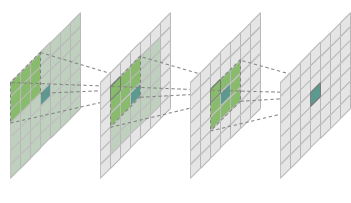
\includegraphics[width=0.7\linewidth]{images/methods_hybrid/field_of_view.png}
    \captionsetup{justification=justified, singlelinecheck=false, width=1\linewidth, labelfont=bf} 
    \caption[]{Figure demonstrating how the use of repeated convolution operations can process global information. The center of the 7x7 grid is marked with ocean color, and it represents an entity in the Lux environment. The increasing field of view is indicated by the shaded green area. The image shows how both local and global information can be utilized in the generation of the entity's action.}
    \label{fig:field_of_view}
\end{figure}

\begin{figure}[htbp]
    \centering
    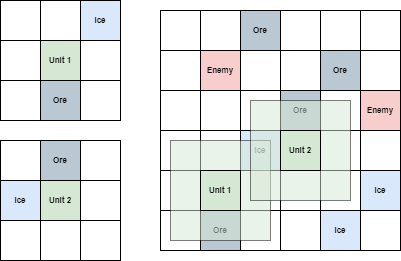
\includegraphics[width=0.7\linewidth]{images/methods_hybrid/feature_extractor/map.png}
    \captionsetup{justification=justified, singlelinecheck=false, width=1\linewidth, labelfont=bf} 
    \caption[]{Figure showing how performing shape-preserving convolution operations on the whole observed map (right) is similar to having localized observations for every unit (left). The image represents a segment of the observed game board. The range of a 3x3 convolution around the units can be seen on the right, marked by an opaque green filter.}
    \label{fig:map}
\end{figure}

\bigskip

\noindent Because a central decision maker is used, but in a way that allows each agent to make their decisions based on their \textbdd{localized observations}, similarly to a distributed method, we call this approach \textbdd{hybrid}. Later, we augment this method with the ability to \textbdd{assign rewards to individual} factories and units instead of purely global rewards. This change makes our approach more similar to a truly multi-agent control system while maintaining the benefits of operating with a \textbdd{single global observation} of the game board. We will compare this modified reward-assignment method to the original global reward system. For a more detailed comparison of the mentioned methods, please refer to \autoref{tab:hybrid-table}.

\bigskip

\noindent The training goal remained consistent for this phase as well: \textbdd{learn how to keep factories alive} until the end of the episode. We will now outline the specifications of the training algorithm and model used in the test.

\begin{table}[htbp]
    \centering
    \begin{tabularx}{\linewidth}{|Y|C{2.3cm}|C{2.3cm}|C{2.3cm}|C{2.3cm}|C{2.3cm}|}
        \toprule
        \textbf{Property} & \textbf{Monolithic} & \textbf{Distributed with Local Observations} & \textbf{Distributed with Global Observations} & \textbf{Hybrid with Global Trajectories} & \textbf{Hybrid with Separate Trajectories} \\
        \midrule
        Passes through Model & once & per agent & per agent & once & once \\
        \midrule
        Features Stored & once & per agent & per agent & once & once \\
        \midrule
        Stored Feature Size & global & local & global & global & global \\
        \midrule
        Field of View & global & local & global and local & global and local & global and local \\
        \midrule
        Distributed Rewards & no & yes & yes & no & yes \\
        \midrule
        Handles Changing Agent Numbers & yes & no & no & yes & yes \\
        \bottomrule
    \end{tabularx}
    \captionsetup{justification=justified, singlelinecheck=false, width=1\linewidth, labelfont=bf} 
    \caption{Table showing the differences between agent control architectures. While storing global observations for every agent with a distributed approach is similar to the hybrid architecture, it requires much more memory and cannot handle changing agent numbers. A hybrid architecture with separating trajectories (\autoref{subsec:grouping}) has every benefit of distributed control.}
    \label{tab:hybrid-table}
\end{table}

\subsection{Environment}

\noindent The environment largely aligns with the description in \autoref{subsec:mono-environment}, with notable changes made to the action space. It now encompasses \textbdd{all actions available} in the Lux AI environment (\autoref{subsec:lux-action}), with a few exceptions, detailed in \autoref{subsec:actions}. Additionally, a \textbdd{stricter action masking} mechanism has been applied to limit unnecessary movements and collisions among units.

\subsection{Heuristic Bidding and Factory Placement}

\noindent We retained our initial Gaussian factory placement heuristic outlined in \autoref{subsec:heur-bidding-factory}, making minor adjustments to the weighting calculation and scale of the Gaussian filters to ensure factories are positioned \textbdd{as close as possible to ice}.


\subsection{Actions} \label{subsec:actions}

\noindent Since our goal is to keep the factories alive until the end of the game, we decided to \textbdd{get rid of the lichen mechanic} completely via action masking. This meant that the factories had three possible actions left: build heavy, build light, and do nothing. We forbade the self-destruct action for units since hostility was not needed to achieve the simplified objective.

\bigskip

\noindent Unit actions are comprised of an action type and action settings, depending on the type. Most action settings were implemented heuristically, such as the transfer amount and the repeat flag; however, the most significant parameters were left for the model to decide. Parameters include the move direction, pickup amount, transfer direction, and transfer resource.

\bigskip

\noindent We \textbdd{forbade illegal actions}, such as factory actions that require more resources than the factory's current cargo, moving out of the map, and choosing unit actions that need more power than the agent's current battery. Actions that would slow down exploration were also disabled to \textbdd{speed up the training}. Such actions are doing nothing when the factory could be producing heavy units with its resources, units recharging, or picking up power from factories while at full power. Agent collisions between the team members were also disabled, with keeping track of each unit's movement possibilities and allowing only one at a time to step on a board tile. To stop factories from spawning new units on top of existing ones, agent creation is masked out if a unit is standing on the middle tile of a factory. Agents cannot enter the middle of factories once they have stepped away from them. Actions we considered too complex and unnecessary for the game were also removed with masking, such as picking up resources from factories and transferring resources or power to other agents. The complete list of possible actions and their requirements can be found in \autoref{tab:actions}.

\begin{table}[htbp]
    \centering
    \begin{tabular}{p{1.5cm}|p{3cm}|p{3cm}|p{6cm}}
        \hline
        Entity & Action & Parameters & Requirements \\
        \hline
        Factory & Build Heavy unit & None & - 100 metal in factory \newline - 500 power in factory \newline - middle of factory is empty \\
        \hline
        Factory & Build Light unit & None & - 10 metal in factory \newline - 50 power in factory \newline - middle of factory is empty \\
        \hline
        Factory & Do nothing & None & - no resources to build heavy unit \\
        \hline
        Unit & Do nothing & None & - no power to update action queue \\
        \hline
        Unit & Recharge & Amount [0, 10] & - battery not full \\
        \hline
        Unit & Pickup & Amount [0, 10] & - battery not full \newline - standing on factory \\
        \hline
        Unit & Move & Direction [0, 4] & - no friendly unit at target \newline - enough power \newline - no enemy factory at target \\
        \hline
        Unit & Transfer & Direction [0, 5] \newline Resource [0, 1] & - has cargo \newline - target is factory \\
        \hline
        Unit & Dig & None & - standing on ice, ore or rubble \newline - enough power \\
        \hline
    \end{tabular}
    \captionsetup{justification=justified, singlelinecheck=false, width=1\linewidth, labelfont=bf}
    \caption{Table containing the list of possible actions, along with their requirements. If the requirements are not fulfilled, the action is masked out.}
    \label{tab:actions}
\end{table}


\subsection{Observation}

\noindent We maintained the observation space described in \autoref{subsec:mono-observation}, as it already covered the necessary information for the feature extractor model to align agents for ice resource collection and survivability. Although additional \textbdd{location information} was provided to the network, it was only utilized for \textbdd{auxiliary purposes} and filtering, not incorporated into the forward pass of the feature extractor.

\subsection{Trajectory Separation} \label{subsec:grouping}

\noindent In a \textbdd{multi-agent environment}, where the actions of units and factories are deeply intertwined, the question of \textbdd{credit assignment} naturally arises. Suppose we use rewards corresponding to a global objective or to objectives that require the cooperation of multiple units or factories. In such a scenario, tracking whom to reward and what amount is challenging since multiple agents work towards a common goal. A \textbdd{centralized control} approach offers a potential solution, as all units and factories will belong under a single agent, which receives a \textbdd{global reward} after performing the actions with all entities. Such reward assignment is still possible when using a fully multi-agent approach by giving every agent the sum or mean reward of the team. \label{par:global-rew} However, as we will later see, relying purely on global rewards makes it \textbdd{hard for the model to learn} which entity's action was beneficial from the \textbdd{many numbers of entities}. The more entities we have, the \textbdd{less of a chance} there is that most of them \textbdd{behave optimally}. A highly beneficial or detrimental action can skew the total reward, which can lead to the \textbdd{reinforcement of bad behavior} or the \textbdd{punishment of good behavior} for the entities whose reward was less dominant in the final sum.

\bigskip

\noindent To tackle this complex problem, we use rewards that can be \textbdd{immediately credited} to the performing or benefiting entity. The ice-dug reward is credited to the performing unit, while the ice-transfer reward is split between the performing unit and the receiving factory. Instead of summing up these rewards to a single global value, we \textbdd{store them separately} to track which entities' actions resulted in how much reward. Since we are using an actor-critic method for training, the critic values should also be distributed. We utilize separate critic value predictions for each entity (\autoref{sec:hybrid-network-actor-critic}). These separate predictions are generated using information about the whole game state, similar to the method of \cite{lowe2020multiagent}.

\bigskip

\noindent In addition to \textbdd{global} and \textbdd{per-entity} reward assignments, we also experimented with putting entities into \textbdd{groups} according to certain grouping rules, where a group's reward is the sum of its members' reward. An example of the reward separations between different groups can be seen in \autoref{fig:rewards}.

\bigskip

\noindent Similar to the rewards and critic values, we also store the action log probabilities and entropies separately. This separation essentially splits every environment step into \textbdd{multiple training examples}, creating multiple \textbdd{distinct trajectories} from the same number of environment steps. The loss calculation does not change from the original PPO algorithm, as the modification simply translates into an additional tensor dimension, and all of the loss samples will get averaged into a single loss value as shown on \autoref{fig:policy-loss}. After the modification, during backpropagation, the \textbdd{weights can be updated more accurately} to reinforce good and diminish bad behavior since the fewer units and factories that belong to one group, the less of a chance a single entity has of \textbdd{skewing their group's reward}, resulting in an inaccurate advantage calculation and a faulty weight update. We will refer to this method as \textbdd{trajectory separation}.

\begin{figure}[htbp]
    \centering
    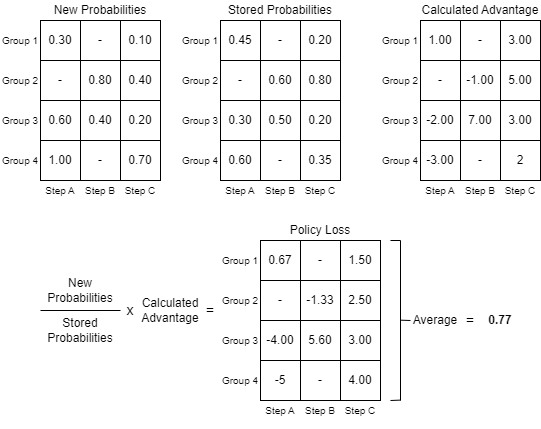
\includegraphics[width=0.7\linewidth]{images/methods_hybrid/trajectory_separation/policy_loss.png}
    \captionsetup{justification=justified, singlelinecheck=false, width=1\linewidth, labelfont=bf} 
    \caption[]{Demonstrating policy loss calculation with the extended dimension. The probabilities and advantages are calculated on a group level. The matrices on the image represent a mini-batch consisting of 3 environment steps. Inactive groups at all steps are marked with a dash, as these are excluded from the training data. The loss gets computed for all active groups, creating more training examples. In the above image, three environment steps resulted in 9 train steps. These loss values are then averaged to get a final scalar loss value. For simplicity, the clipping operation and advantage normalization are left out of this image.}
    \label{fig:policy-loss}
\end{figure}

\begin{figure}[htbp]
    \centering
    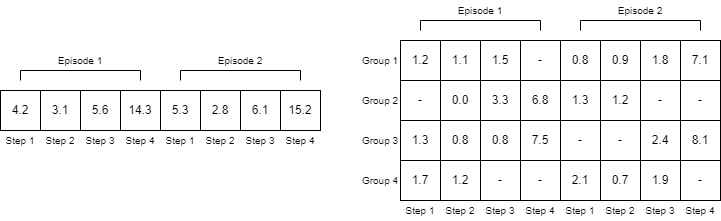
\includegraphics[width=0.8\linewidth]{images/methods_hybrid/trajectory_separation/rewards.png}
    \captionsetup{justification=justified, singlelinecheck=false, width=1\linewidth, labelfont=bf} 
    \caption[]{Image showing the difference between global rewards (left) and rewards distributed into groups (right). The examples are 4-length episodes with random data.}
    \label{fig:rewards}
\end{figure}

\bigskip

\noindent The PPO algorithm uses a \textbdd{termination flag} stored for every step when calculating future rewards during advantage estimation. This flag signals the start of a \textbdd{new episode} and ensures we do \textbdd{not include} this episode's rewards in the \textbdd{cumulative return} calculation of the previous steps. We need to modify this by adding an \textbdd{extra dimension} to the stored termination flag tensor in order to keep track of the lifecycle of every group since we do not want to calculate steps into the cumulative return where the \textbdd{group was inactive}. An example can be seen on \autoref{fig:dones}. A group is marked done when it contains no active units or factories. In the simplest case, when the groups consist of single units and factories, the flag is set to True if the entity: 1. has not been created yet, 2. is destroyed at that step, or 3. remains destroyed. A group consisting of multiple entities can be calculated by performing the \textbdd{AND} operation on each of its member's termination flags. At the first step of an episode, every group is marked done.

\begin{figure}[htbp]
    \centering
    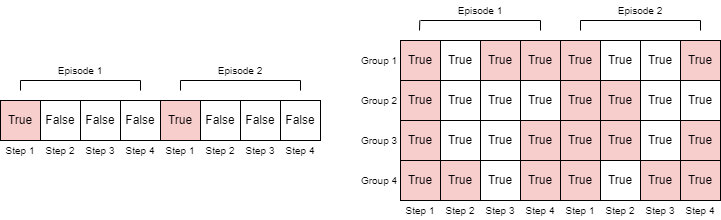
\includegraphics[width=0.8\linewidth]{images/methods_hybrid/trajectory_separation/dones.png}
    \captionsetup{justification=justified, singlelinecheck=false, width=1\linewidth, labelfont=bf} 
    \caption[]{Image showing termination flags for a standard environment (left) and termination flags stored for every group (right). In addition to flagging the end of an episode, the death of a group is also indicated. The examples are 4-length episodes with random data. The cells with true values were given red backgrounds for visibility.}
    \label{fig:dones}
\end{figure}


\noindent If we use a grouping rule that allows groups to be occasionally inactive, for example, by assigning every unit or factory to its own group, the number of training examples belonging to one step will \textbdd{not be constant}. Since we divide the \textbdd{mini-batches} by environment step, this could mean that not all \textbdd{mini-batches} consist of the \textbdd{same number of training examples}. Because the loss values are averaged over a mini-batch to get the final loss, this could mean that training examples that belong to steps with fewer active groups have a \textbdd{more dominant} effect during gradient updates since, on average, they create mini-batches with fewer training examples. Following the same logic, entities at more populated steps of the environment will have \textbdd{less impact} on the final loss. We test using grouping rules that \textbdd{keep group numbers consistent} to overcome this effect. We also experimented with keeping all entity trajectories separate but kept \textbdd{only a set number of training examples} from each step to reduce the training example variance.


\subsection{Feature Extractor Model}
\label{sec:hybrid-network-architecture}

\noindent We use a \textbdd{convolutional neural network} to map the observations into actions for each unit and factory on the board and to output critic values and log probabilities used by the training algorithm. Both the \textbdd{Actor} and \textbdd{Critic} networks have the same \textbdd{Embedding Network} but do not share the weights to avoid the competing objectives of the policy and value functions (\cite{shengyi2022the37implementation}). The structure of the embedding can be seen on \autoref{fig:embedding}. The main building blocks of the network are convolutional layers with \textbdd{3x3 kernels} and padding to \textbdd{keep the board's shape}. The layers alternate between a basic convolutional layer and a \textbdd{residual connection} (\autoref{subsec:residual}), where two convolutional layers are followed by a \textbdd{Squeeze-and-Excitation} block (\autoref{subsec:se}). Each convolutional layer's output goes into a two-dimensional \textbdd{batch normalization} block (\autoref{subsec:batchnorm}), then to a \textbdd{Leaky ReLU} (\autoref{subsec:leaky-relu}) activation function. The weights of the convolutional layers are scaled by their \textbdd{spectral norm} (\autoref{subsec:spectralnorm}). We also implemented the same weight downscaling outlined in \autoref{subsec:weight-scaling}.

\begin{figure}[htbp]
    \centering
    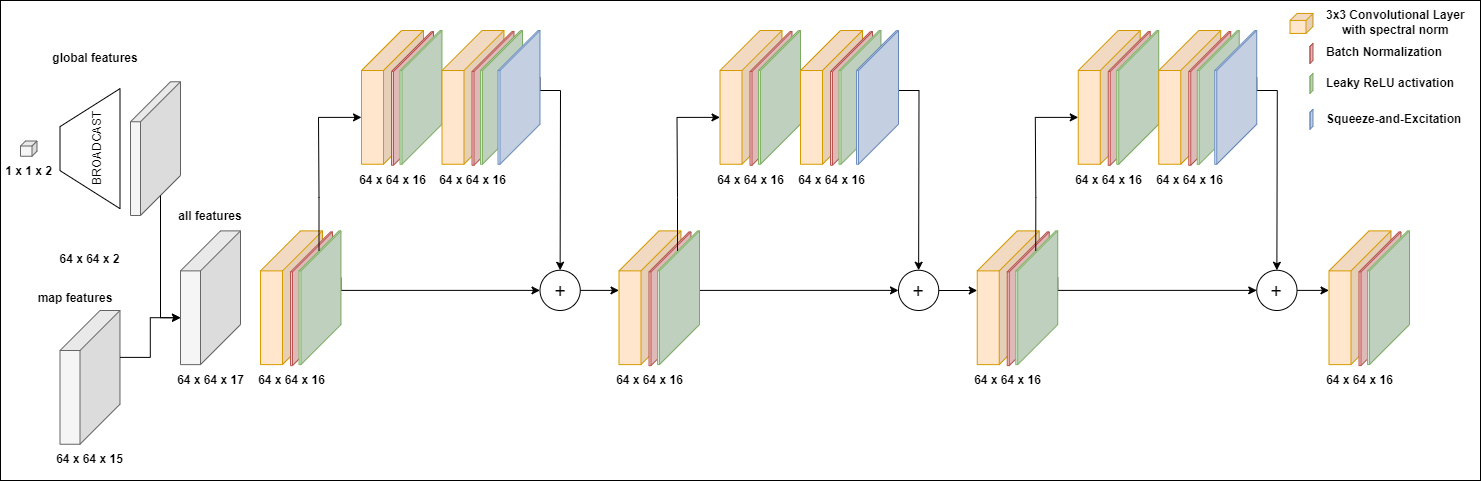
\includegraphics[width=1\linewidth]{images/methods_hybrid/feature_extractor/embedding.png}
    \captionsetup{justification=justified, singlelinecheck=false, width=1\linewidth, labelfont=bf} 
    \caption[]{The structure of the Embedding network. The network uses convolutional layers with 3x3 kernels. Each convolutional block is followed by 2D batch normalization and a Leaky ReLU activation function (\autoref{subsec:leaky-relu}). In order to regularize the network output and allow more layers, we use residual connections with a Squeeze-and-Excitation layer output. This embedding is the backbone of the critic and actor network.}
    \label{fig:embedding}
\end{figure}

\subsection{Actor and Critic}
\label{sec:hybrid-network-actor-critic}

\noindent After the embedding is created from observations, the critic values and the actions are constructed by their respective heads. The Lux environment is highly complex, and the entities need to solve multiple tasks in order to reach their goal. Therefore, multiple reward sources (\autoref{subsec:hyb-rew}) are needed to ensure the rewards are not too sparse for optimal training. In addition to that, since the entities get rewarded based on outcomes, which in reality do not entirely depend on them, it is hard to predict an accurate critic value. Since multiple critic heads already proved to be successful in multi-task environments (\cite{mysore2022multicritic}), we decided to provide a separate critic value prediction for each entity and, in addition to that, provide two additional critic heads for both units and factories, respectively, that use global information for their predictions. The \textbdd{Critic Network} (\autoref{fig:critic}) is made up of 4 components: a \textbdd{unit} and a \textbdd{factory} value network that outputs a value at every board position, and a unit and factory \textbdd{global value} network that, in addition to outputting a value for every position, averages them into a single scalar value. The global unit and factory value scalars are then added to every position of the unit and factory value net output, respectively. This structure ensures that each unit and factory's value calculation is based on \textbdd{both local and global} information. The final output values are created by selecting the predicted value at each unit's and factory's position on the board and then adding the value to the entity's group (\autoref{subsec:grouping}).

\bigskip

\begin{figure}[htbp]
    \centering
    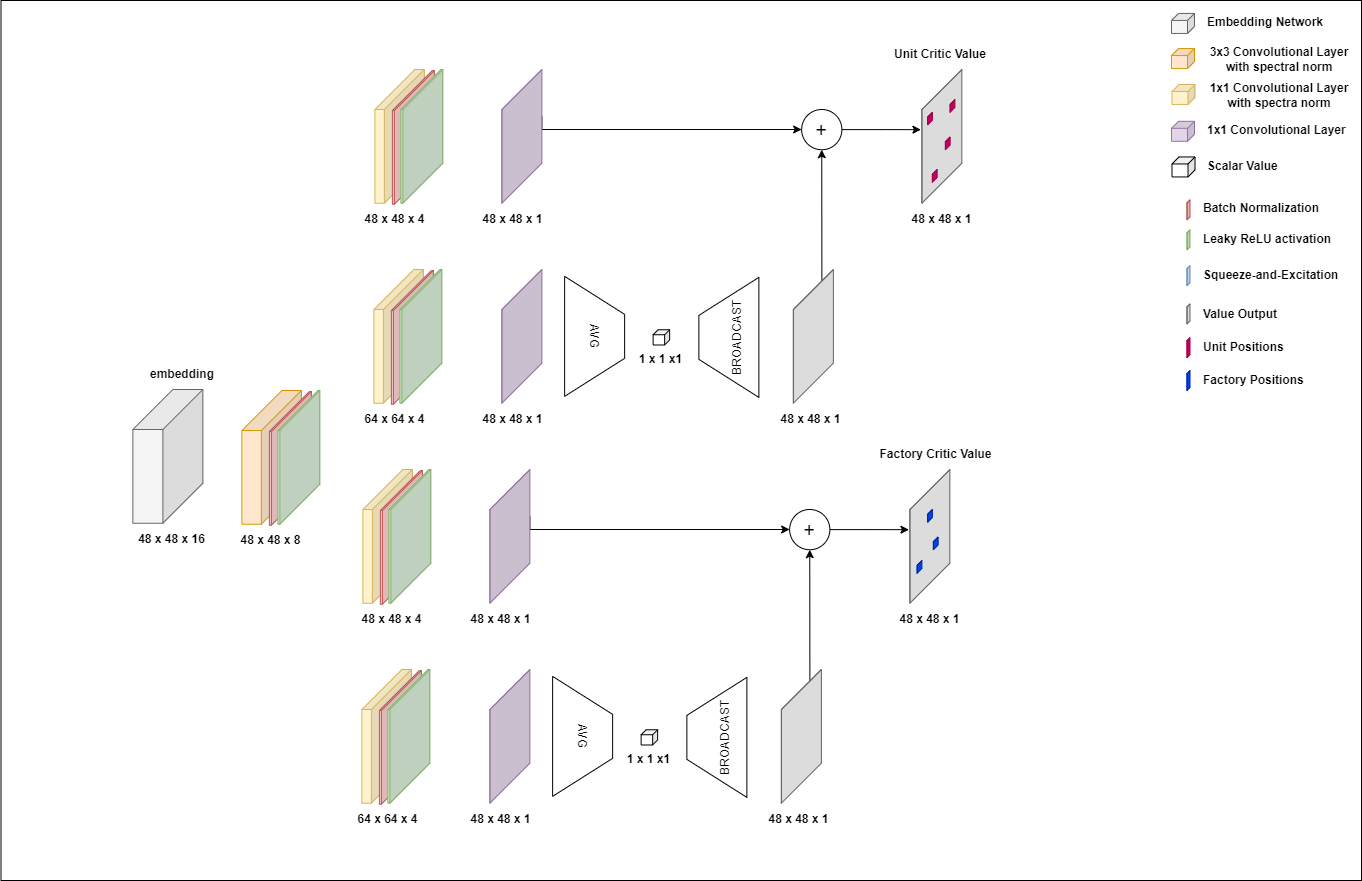
\includegraphics[width=0.9\linewidth]{images/methods_hybrid/actor_critic/critic.png}
    \captionsetup{justification=justified, singlelinecheck=false, width=1\linewidth, labelfont=bf} 
    \caption[]{The Critic network takes the output of the Embedding and outputs critic values for each entity on the board. Each value is comprised of a local value and a global value, which is averaged over the whole board and then added to each position.}
    \label{fig:critic}
\end{figure}

\noindent Actions are created by the \textbdd{Actor Network} (\autoref{fig:actor}). Factories and units have different action spaces, so different actor heads output their actions. The action space of the factories is a simple discrete action space, while the units have a \textbdd{multi-dimensional action space}, where each action has a different set of parameters. Due to some actions having a \textbdd{heuristic parameterization} (\autoref{subsec:actions}), only four parameter action heads are used in addition to the action type head. The heads output log probabilities, which are then used to create \textbdd{categorical distributions} (\cite{categorical}), discrete probability distributions over the possible actions. Actions are sampled from these distributions after setting the probability of masked-out actions to zero. The sampled actions are outputted in the same board shape at the positions of units and factories. For each entity, the composite action's log probability and the distributions' entropies are summed together at an entity level. These values are added to the total log probability and entropy of the given entity's group (\autoref{subsec:grouping}).

\begin{figure}[htbp]
    \centering
    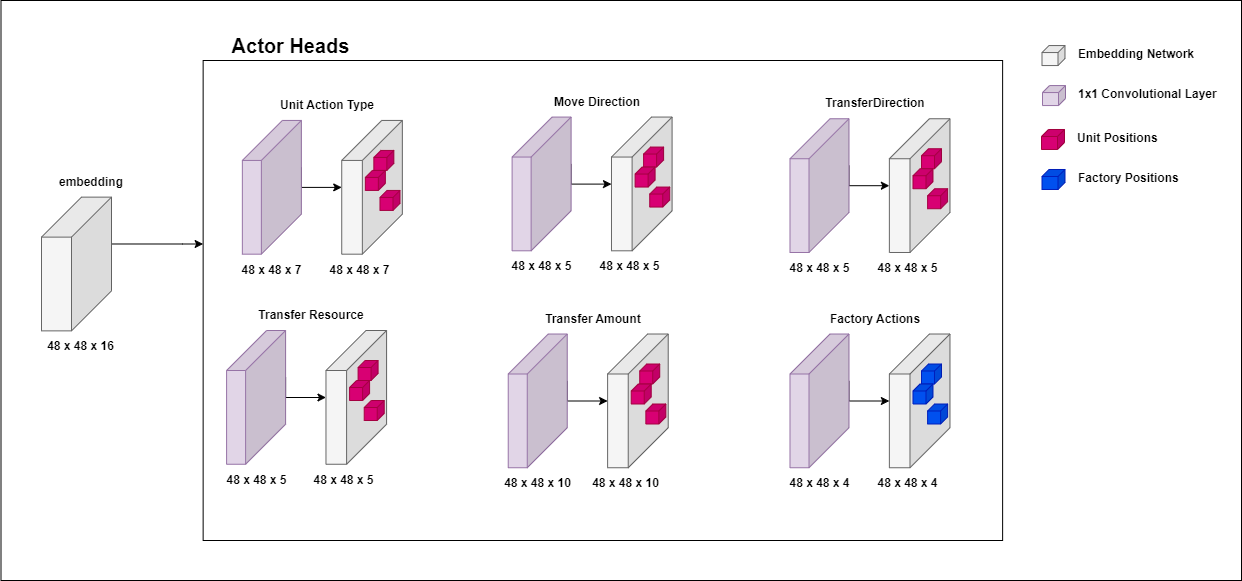
\includegraphics[width=1\linewidth]{images/methods_hybrid/actor_critic/actor.png}
    \captionsetup{justification=justified, singlelinecheck=false, width=1\linewidth, labelfont=bf} 
    \caption[]{The Actor network is made up of separate actor heads, which share the same Embedding network. The output of these heads is the log probabilities of the action distributions. Factory actions have only one output, while unit actions require multiple outputs to parameterize them.}
    \label{fig:actor}
\end{figure}

\subsection{Reward Function}
\label{subsec:hyb-rew}

\noindent The rewards are shaped to \textbdd{encourage the units to bring ice to factories}. In order to achieve this, 1 unit of reward is given after every one water worth of \textbdd{ice is transferred to a factory}. After \textbdd{mining} one water worth of \textbdd{ice}, a $\frac{1}{10}$ unit of reward is given to ensure that units find desirable behavior patterns as early as possible. All of these rewards are then divided by to \textbdd{scale them closer to zero}. In order to incentivize units to fill the factories with ice as early as possible, we utilized the same formulation for the multiplication factor in \autoref{eq:reward-early-scaling}.

\subsection{Training}

\noindent To minimize training duration, we continued utilizing the Masked PPO algorithm (\autoref{subsec:M-PPO}). Our implementation, derived from \cite{luxai_s2-baseline-source}, provided by the contest organizers as a baseline, \textbdd{differes from conventional approaches}. We opted to train the model twice after each rollout step, using data collected from each player separately. This approach enabled us to gather experience from both players without mixing their training examples during mini-batch creation. Leveraging \textbdd{self-play} and access to both enemy and own player data, we halved our rollout size compared to the monolithic approach (\autoref{sec:monolithic-approach-training}) to 4,096 steps. Additionally, we reduced the batch size by a factor of 4, from 1,024 to 256 steps so that we could parallelize more environments. Further details on hyperparameters and subsequent modifications can be found in \autoref{app:c}.

\subsection{Evaluation} \label{sec:hybrid-metrics}

\noindent The evaluation settings remained consistent with those outlined in the monolithic approach (\autoref{sec:monolithic-approach-eval}), except employing 12 evaluation environments. The episode lengths was set to the maximum value of 1,000 steps. While episode length serves as a primary metric reflecting our training goal, measuring the \textbdd{amount of ice transferred by units to factories} provides a more nuanced comparison, as it is practically unbounded, unlike episode length, which can be quickly reached in multiple trials. Additionally, we recorded other metrics, such as the \textbdd{average factory count per step}, to assess the ability of entities to maintain multiple functioning factories instead of just one. Most other metrics were retained as baselines for comparison.
